%%%%%%%%%%%%%%%%%%%%%%%%%%%%%%%%%%%%%%%%%
% Beamer Presentation
% LaTeX Template
% Version 1.0 (10/11/12)
%
% This template has been downloaded from:
% http://www.LaTeXTemplates.com
%
% License:
% CC BY-NC-SA 3.0 (http://creativecommons.org/licenses/by-nc-sa/3.0/)
%
%%%%%%%%%%%%%%%%%%%%%%%%%%%%%%%%%%%%%%%%%

%------------------------------------------------------------------------------%
%	PACKAGES AND THEMES
%------------------------------------------------------------------------------%

\documentclass{beamer}

%%% From template

\usepackage[intoc]{nomencl}

\textwidth=6in \oddsidemargin=0.5in \topmargin=-0.5in
\textheight=9in  % 9in must include page numbers
\textfloatsep = 0.4in \addtocontents{toc}{\vspace{0.4in} \hfill
Page\endgraf} \addtocontents{lof}{\vspace{0.2in} \hspace{0.13in} \
Figure\hfill Page\endgraf} \addtocontents{lot}{\vspace{0.2in}
\hspace{0.13in} \ Table\hfill Page\endgraf}

% We've already imported some of the most commonly used packages for inserting
% formulas, images, tables, and references.
% If you need more, you can find a list of Latex packages
% here: https://www.ctan.org/pkg/

%\usepackage{textcomp}
\usepackage{array}
\usepackage{listings}
\usepackage{setspace}
%\usepackage{mathptmx}
\usepackage[table, svgnames]{xcolor}
\usepackage{colortbl}
\usepackage{graphicx}
\usepackage{amssymb,amsmath}
\usepackage{subfig}
\usepackage{epsfig}
\usepackage{times}
\usepackage{float}
\usepackage{rotating}
\usepackage{makeidx}
\usepackage{url}
\usepackage{multirow}
\usepackage{booktabs}
\usepackage{tabularx}

\usepackage[subfigure,titles]{tocloft}
\usepackage{acronym}
\usepackage{datetime}

%%another algorithm package
\usepackage{algorithm}
\usepackage{algorithmic}

\makenomenclature

\graphicspath{{Figures/}}
\DeclareGraphicsExtensions{.pdf,.jpeg,.png,.PNG,.eps,.tiff}

\urlstyle{same}

\usepackage{makecell}
\usepackage[nottoc]{tocbibind}
\usepackage{titletoc}
\usepackage{sfchap}
\usepackage{sfsection}
\usepackage[authoryear]{natbib}
%\usepackage{apacite}
\usepackage{appendix}
%\usepackage{tocbibind}

%\usepackage[nottoc]{tocbibind}
\setcounter{secnumdepth}{7}
\setcounter{tocdepth}{7}

\usepackage{tikz}
\usetikzlibrary{shapes.geometric,arrows}
\tikzstyle{box} = [ rectangle, rounded corners, minimum width = 10em, %
                    minimum height = 3em,text centered, draw = black, %
                    fill = blue!20 ]
\tikzstyle{arrow} = [thick,->,>=stealth]

\usepackage{hyperref}
\hypersetup{
  pdftitle={A LaTeX Format for Theses and Dissertations},
  pdfauthor={Eli Hooten},
  bookmarksnumbered, %Determined if chapter numbers are included in the bookmark list
  pdfstartview={FitH},
  pdfborder={0 0 0},
  plainpages=false
}
\usepackage[all]{hypcap}

% Prevent double spaced equations
\newenvironment{tightequation}{\singlespace\begin{equation}}{\end{equation}}

% Extra junk to pretty up the table of contents
\setlength{\cftsecnumwidth}{2.8em}
\setlength{\cftsubsecnumwidth}{3.7em}
\setlength{\cftsubsubsecnumwidth}{4.6em}
\setlength{\cftparanumwidth}{5.5em}
\setlength{\cftsubparanumwidth}{6.5em}
\setlength{\cfttabnumwidth}{3.5em}
\setlength{\cftfignumwidth}{3.5em}

% Prevents the splitting of long footnotes across multiple pages.
% Use with caution.
\interfootnotelinepenalty=10000

\usepackage[T1]{fontenc}
\usepackage{lmodern}
\newcommand\Fontvi{\fontsize{9}{9.2}\selectfont}

%% From Accretion Shock paper
%------------------------------------------------------------------------------%
% Packages

%\usepackage{amsmath}
\usepackage{aasmacros} % For journal symbols
\usepackage{duckuments} % For the ducks
\usepackage{soul} % To strike out multiple lines

%% From methods paper
% Define \bigtimes, taken from
% https://tex.stackexchange.com/questions/202527/writing-x-as-a-symbol-with-limits
\DeclareFontFamily{U}{mathx}{\hyphenchar\font45}
\DeclareFontShape{U}{mathx}{m}{n}{
      <5> <6> <7> <8> <9> <10>
      <10.95> <12> <14.4> <17.28> <20.74> <24.88>
      mathx10
      }{}
\DeclareSymbolFont{mathx}{U}{mathx}{m}{n}
\DeclareFontSubstitution{U}{mathx}{m}{n}
\DeclareMathSymbol{\bigtimes}{1}{mathx}{"91}

%%% From template

\renewcommand{\nomname}{LIST OF ABBREVIATIONS}

% Stats table label
\newcommand{\statslabel}[2]{\multirowcell{#1}[-1.6mm][c]{#2}}

% Below heading rule.
\newcommand{\otoprule}{\midrule[\heavyrulewidth]}

\renewcommand{\contentsname}{TABLE OF CONTENTS}
\renewcommand{\listfigurename}{LIST OF FIGURES}
\renewcommand{\listtablename}{LIST OF TABLES}
\renewcommand{\bibname}{ \texorpdfstring{{References\vspace{10mm}}}{References}   }
%
\renewcommand{\chaptermark}[1]{%
  \markboth{\MakeUppercase{%
      \chaptername}\ \thechapter.%
    \ #1}{}}

%%% From Accretion Shock Paper
%------------------------------------------------------------------------------%
% Results
\newcommand{\PeriodRatioGRoverNRxiA}{1.19}
\newcommand{\PeriodRatioGRoverNRxiB}{1.15}
\newcommand{\PeriodRatioGRoverNRxiC}{1.22}
\newcommand{\PeriodRatioGRoverNRxiD}{1.29}
\newcommand{\GrowthRateRatioGRoverNRxiA}{0.96}
\newcommand{\GrowthRateRatioGRoverNRxiB}{0.79}
\newcommand{\GrowthRateRatioGRoverNRxiC}{0.68}
\newcommand{\GrowthRateRatioGRoverNRxiD}{0.47}
\newcommand{\RelDiffAAxiA}{0.29}
\newcommand{\RelDiffAAxiB}{0.14}
\newcommand{\RelDiffAAxiC}{0.05}
\newcommand{\RelDiffAAxiD}{0.17}
\newcommand{\RelDiffACxiA}{0.21}
\newcommand{\RelDiffACxiB}{0.22}
\newcommand{\RelDiffACxiC}{0.10}
\newcommand{\RelDiffACxiD}{0.12}

% Production Codes
\newcommand{\flashx}{\textsc{\texttt{Flash-X}}}
\newcommand{\cocov}{\textsc{CoCoNuT-VERTEX}}
\newcommand{\zelmani}{\textsc{\texttt{Zelmani}}}
\newcommand{\fornax}{\textsc{Fornax}}
\newcommand{\nadafld}{NADA-FLD}
\newcommand{\chimera}{\textsc{Chimera}}
\newcommand{\gmunu}{\texttt{Gmunu}}
\newcommand{\tenet}{\textsc{tenet}}
\newcommand{\spectre}{SpECTRE}

% Math
\newcommand{\p}{\partial}
\newcommand{\pd}[2]{\frac{\partial#1}{\partial#2}}
\newcommand{\td}[2]{\frac{d#1}{d#2}}
\newcommand{\T}{^{\top}}
\newcommand{\mystackrel}[2]{\stackrel{\scriptstyle#1}{\scriptstyle#2}}

% Aliases
\newcommand{\arl}{\mathrm{areal}}
\newcommand{\iso}{\mathrm{iso}}
\newcommand{\wt}{\widetilde}
\newcommand{\etac}{\eta_{\mathrm{c}}}
\newcommand{\rpns}{R_{\textsc{pns}}}
\newcommand{\rsh}{R_{\mathrm{sh}}}
\newcommand{\rac}{R_{\mathrm{ac}}}
\newcommand{\rsc}{R_{\mathrm{Sc}}}
\newcommand{\gammabar}{\overline{\gamma}}
\newcommand{\myeqref}[1]{Eq.~(\ref{#1})}
\newcommand{\thornado}{\texttt{thornado}}
\newcommand{\amrex}{\texttt{AMReX}}
\newcommand{\eos}{EoS}
\newcommand{\cfc}{CFC}
\newcommand{\degrees}{^{\circ{}}}
\newcommand{\mdot}{\dot{M}}
\newcommand{\gr}{\textsc{gr}}
\newcommand{\nr}{\textsc{nr}}
\newcommand{\tauad}{\tau_{\mathrm{ad}}}
\newcommand{\tauac}{\tau_{\mathrm{ac}}}
\newcommand{\tac}{T_{\mathrm{ac}}}
\newcommand{\taa}{T_{\mathrm{aa}}}
\newcommand{\mpns}{M_{\textsc{pns}}}
\newcommand{\bs}[1]{\boldsymbol{#1}}
\newcommand{\mc}{\mathcal}
\newcommand{\bb}{\mathbb}
\newcommand{\appref}[1]{Appendix~\ref{#1}}
\newcommand{\figref}[1]{Figure~\ref{#1}}
\newcommand{\tabref}[1]{Table~\ref{#1}}
\newcommand{\secref}[1]{Section~\ref{#1}}
\renewcommand{\th}{-th}
\newcommand{\nModels}{\repl{5}{7}}
\newcommand{\scipy}{\texttt{scipy}}
\newcommand{\curvefit}{\texttt{curve\_fit}}

\newcommand{\repl}[2]{{}\textbf{#2}}
\newcommand{\Dbar}{\bar{D}}
\newcommand{\Deltabar}{\bar{\Delta}}
\newcommand{\weaklib}{\texttt{weaklib}}
\newcommand{\poseidon}{\texttt{Poseidon}}
\newcommand{\xcfc}{xCFC}
\newcommand{\bc}[1]{\bs{\mc{#1}}}
\newcommand{\wh}{\widehat}
\newcommand{\myol}{\overline}
\newcommand{\bj}{\left(\bs{j}\right)}
\newcommand{\Vshear}{V_{\mathrm{shear}}}
\newcommand{\myne}{n_{\mathrm{e}}}
\newcommand{\myNe}{N_{\mathrm{e}}}
\newcommand{\NK}{N_{K}}
\newcommand{\NSSPRK}{N_{\textsc{ssprk}}}

% Units
\newcommand{\msun}{M_{\odot}}
\newcommand{\erg}{\mathrm{erg}}
\newcommand{\g}{\mathrm{g}}
\newcommand{\cm}{\mathrm{cm}}
\newcommand{\km}{\mathrm{km}}
\newcommand{\s}{\mathrm{s}}
\newcommand{\kb}{k_{\textsc{B}}}
\newcommand{\K}{\mathrm{K}}
\newcommand{\J}{\mathrm{J}}
\newcommand{\ms}{\mathrm{ms}}
\newcommand{\Hz}{\mathrm{Hz}}
\newcommand{\rad}{\mathrm{rad}}

% Colors
\newcommand{\red}[1]{\textcolor{red}{#1}}
\newcommand{\blue}[1]{\textcolor{blue}{#1}}
\newcommand{\magenta}[1]{\textcolor{magenta}{#1}}
\newcommand{\cyan}[1]{\textcolor{cyan}{#1}}
\newcommand{\teal}[1]{\textcolor{teal}{#1}}
\newcommand{\orange}[1]{\textcolor{orange}{#1}}
\newcommand{\green}[1]{\textcolor{green}{#1}}

% Editing
\newcommand{\citeme}{\red{(CITE ME)}}
\newcommand{\sd}[1]{\texttt{\red{(SD: #1)}}}
\newcommand{\ee}[1]{\texttt{\blue{(EE: #1)}}}
\newcommand{\khb}[1]{\texttt{\orange{(KHB: #1)}}}
\newcommand{\KHB}[1]{\texttt{\orange{(KHB: #1)}}}
\newcommand{\am}[1]{\texttt{\cyan{(AM: #1)}}}
\newcommand{\bg}[1]{\texttt{\teal{(BG #1)}}}
\newcommand{\su}[1]{\texttt{\green{(SU #1)}}}


% --- TITLE PAGE SLIDE ---

\title[Dissertation Defense]%
{\thornado-Hydro, xCFC: A Discontinuous Galerkin Hydrodynamics %
Solver for General Relativistic %
Core-Collapse Supernova Simulations}

\author{Samuel J. Dunham}
\date{February 23, 2024}

\begin{document}

\begin{frame}

  \maketitle

  \vspace{-1em}

  \begin{center}
    Eirik Endeve (co-chair), %
    Kelly Holley--Bockelmann (co-chair), \\
    Anthony Mezzacappa, %
    William Gabella, %
    Sait Umar
  \end{center}

\end{frame}

\begin{frame}

  \begin{figure}[ht]
    \centering
    
\includegraphics[width=0.3\textwidth]{fig.thornado_logo.png}
  \end{figure}

  \begin{center}

    \ul{t}oolkit for
    \ul{h}igh-\ul{or}der
    \ul{n}eutrino-r\ul{ad}iation hydr\ul{o}dynamics\\[1em]

  \end{center}

\end{frame}

\begin{frame}
\frametitle{Core-Collapse Supernovae}

  \begin{figure}[htb!]
    \centering
    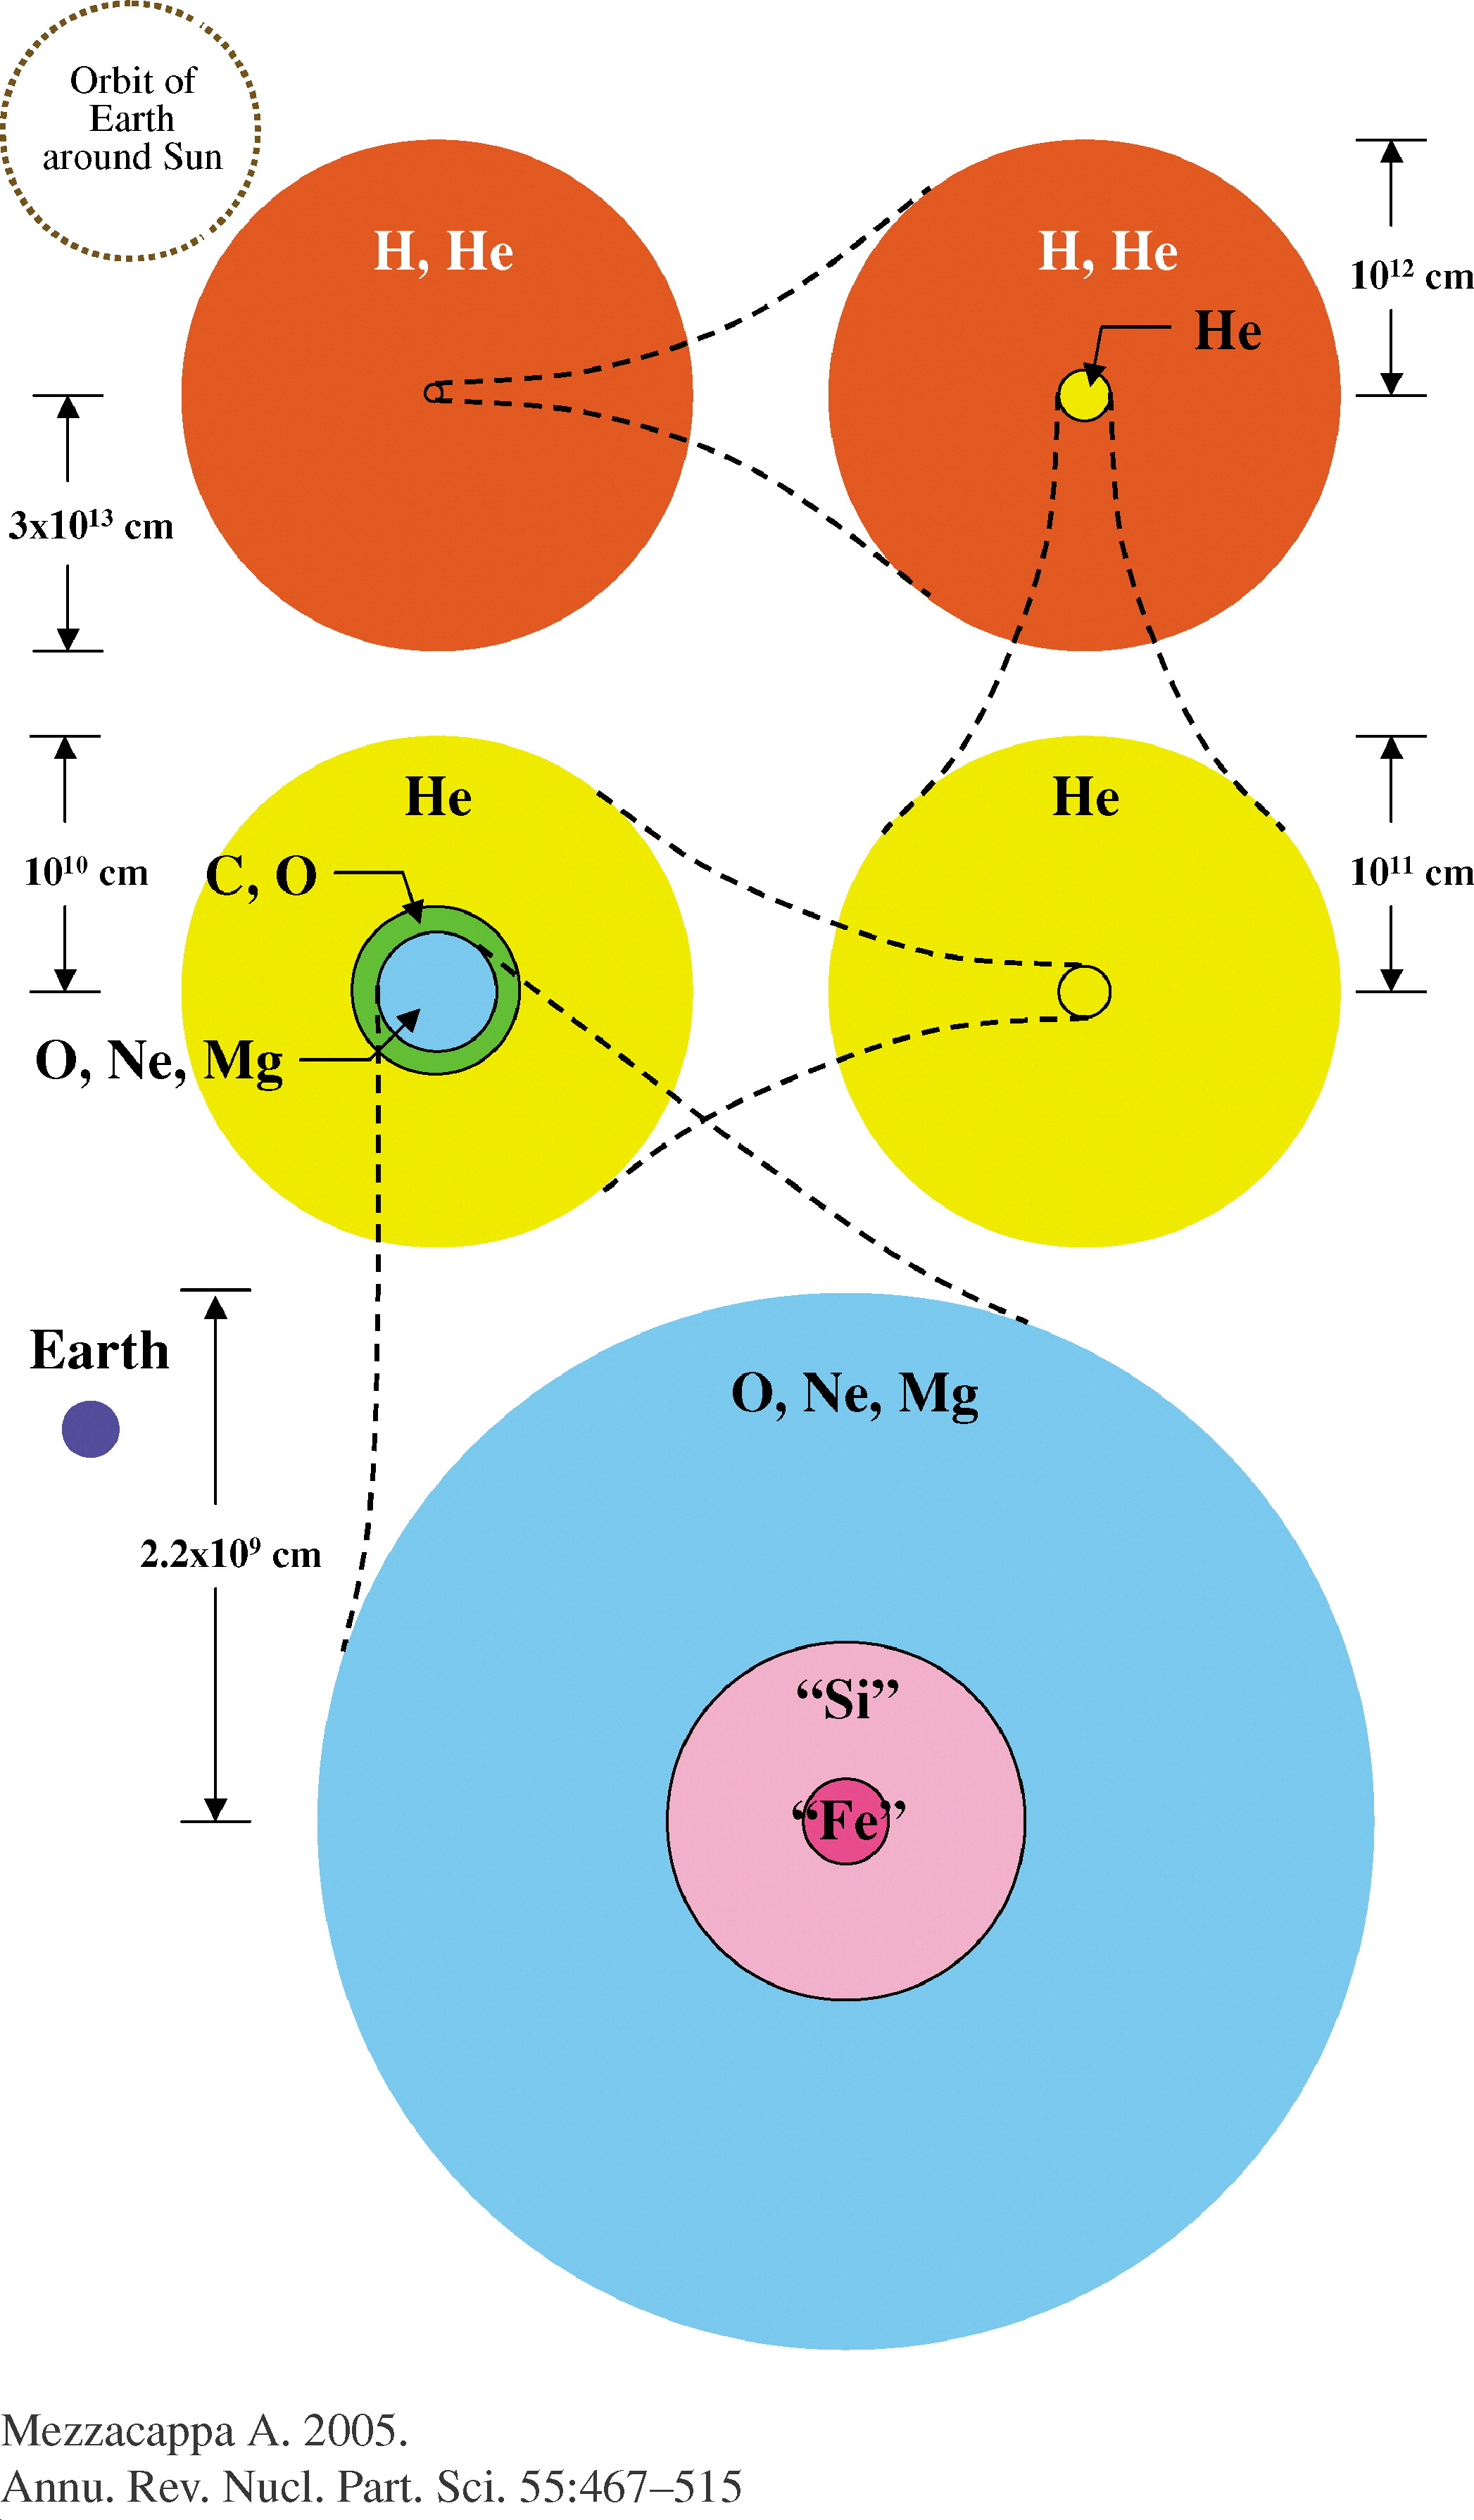
\includegraphics[width=0.35\textwidth]{fig.CCSN_01.jpeg}
  \end{figure}

\end{frame}

\begin{frame}
\frametitle{Core-Collapse Supernovae}

  \begin{figure}[htb!]
    \centering
    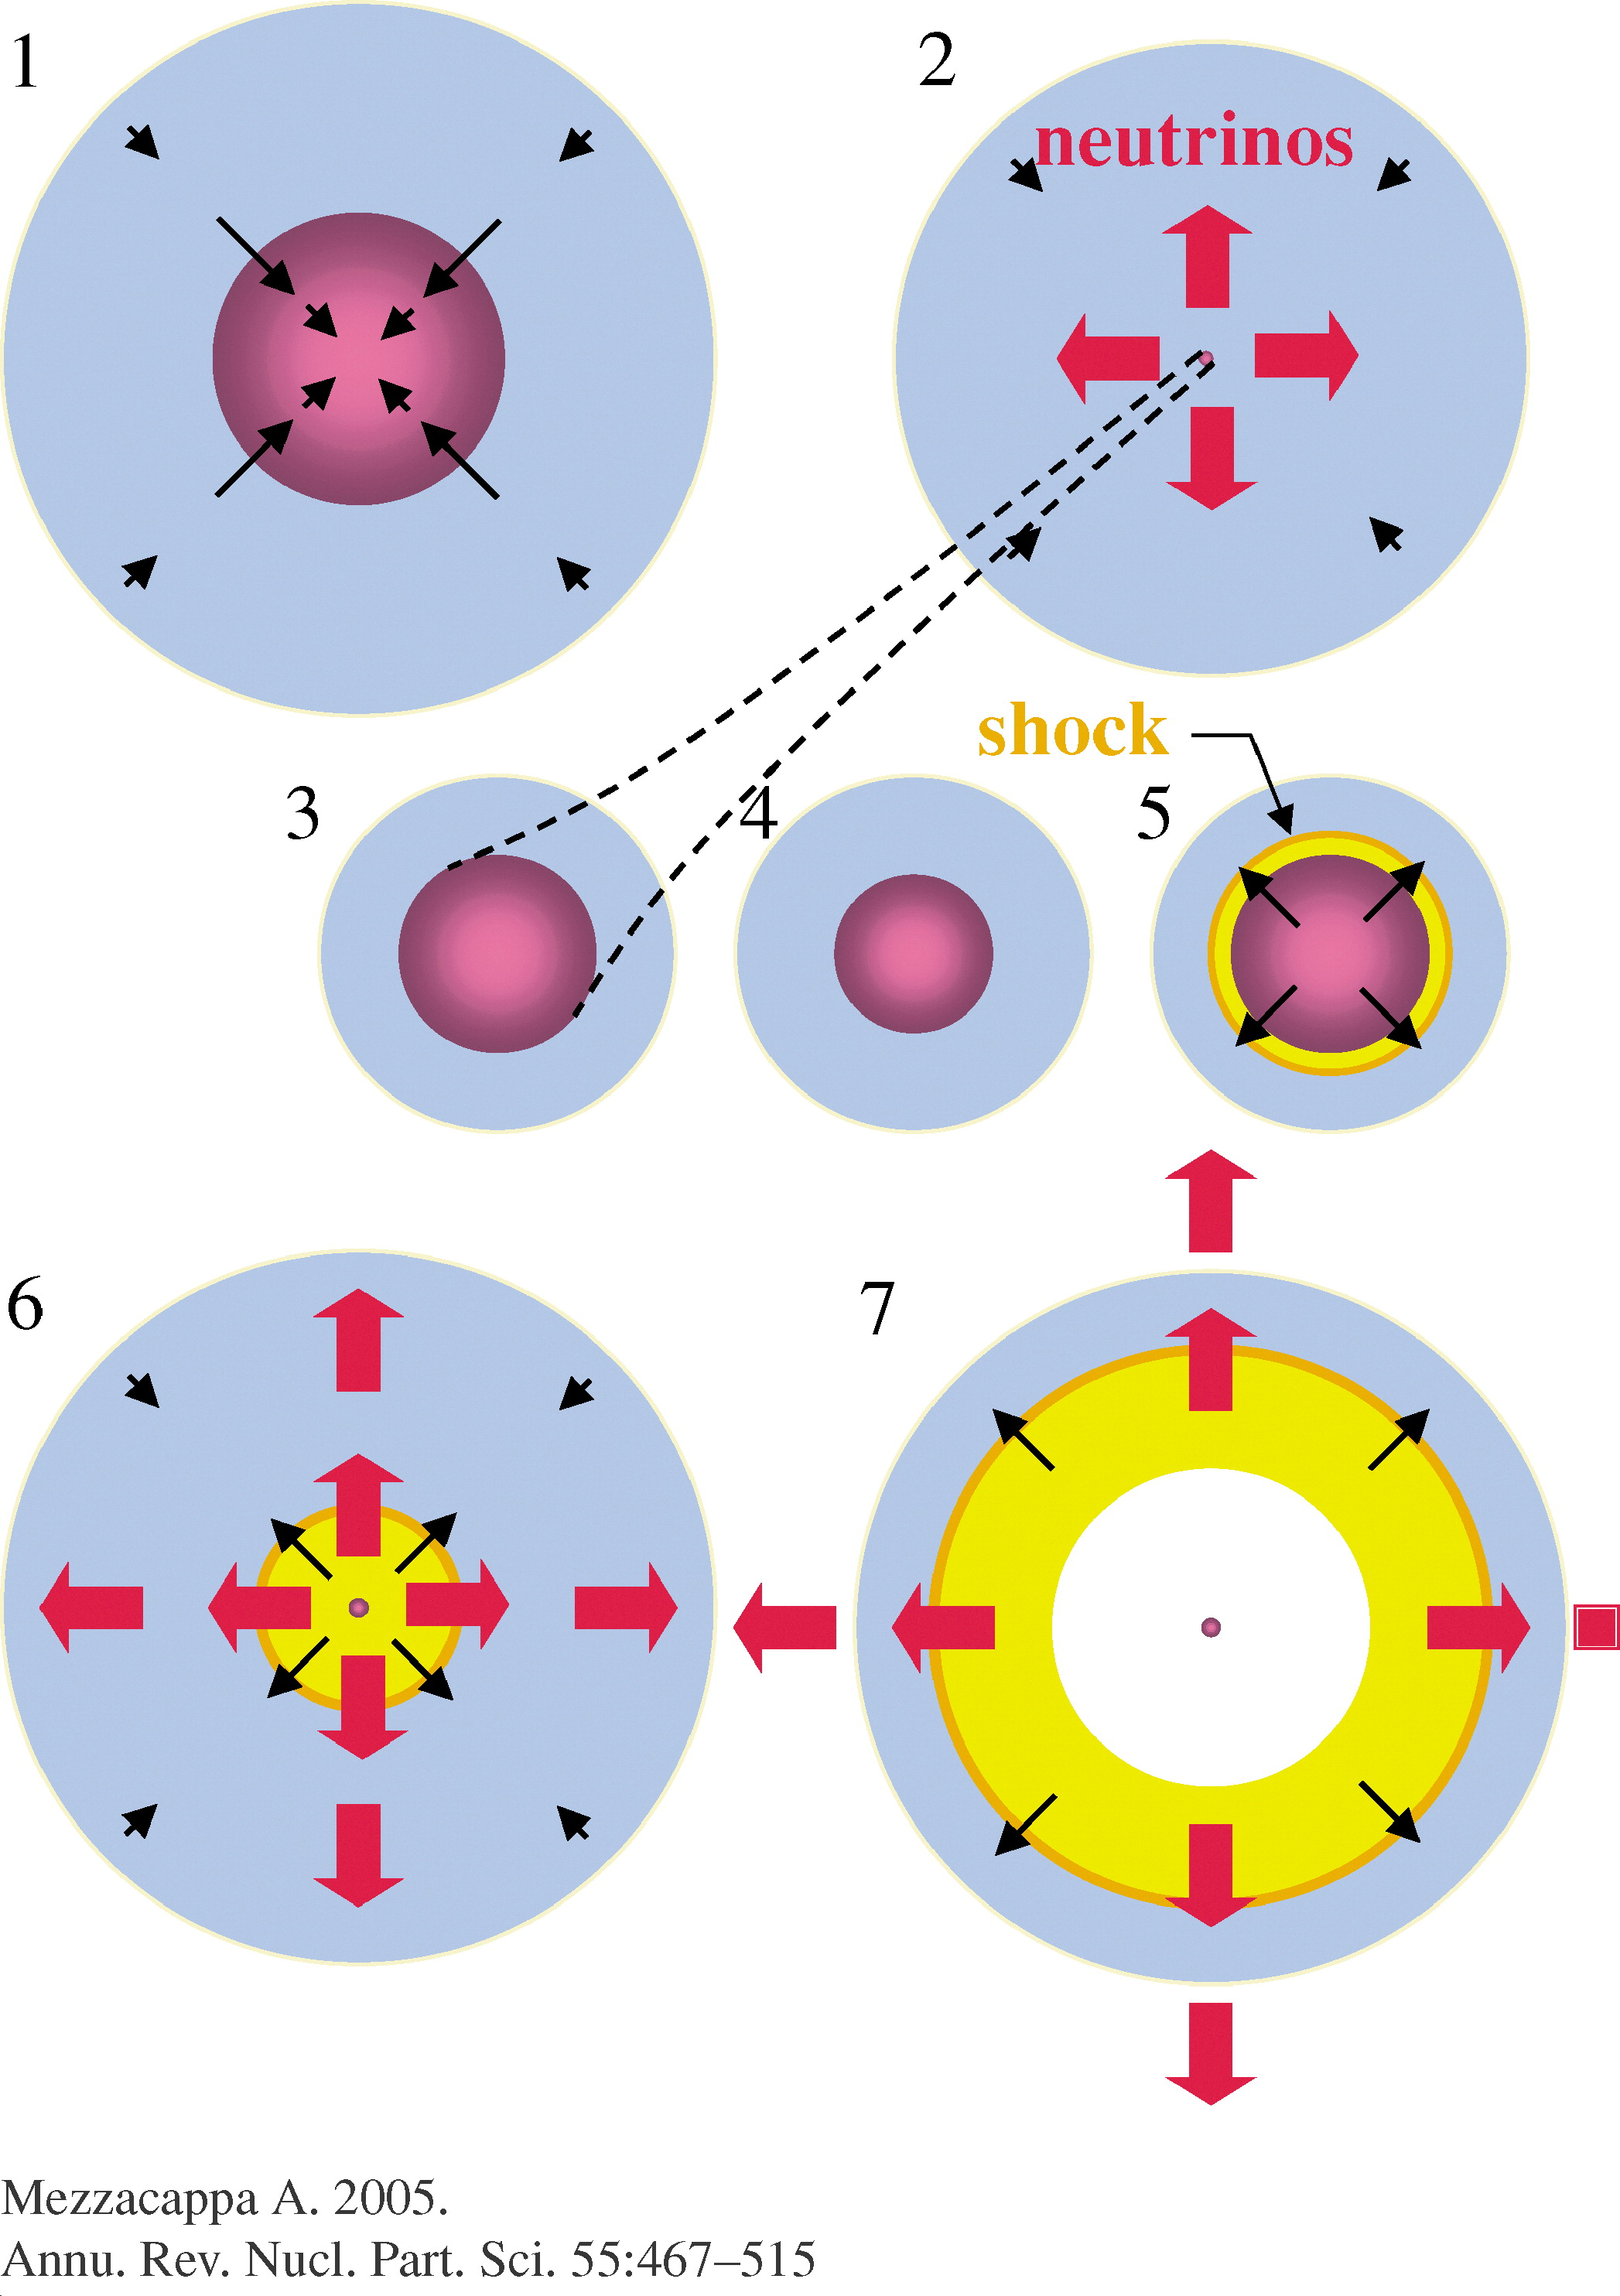
\includegraphics[width=0.4\textwidth]{fig.CCSN_02.jpeg}
  \end{figure}

\end{frame}

\begin{frame}
\frametitle{Historical Interlude}

  \begin{figure}[htb!]
    \centering
    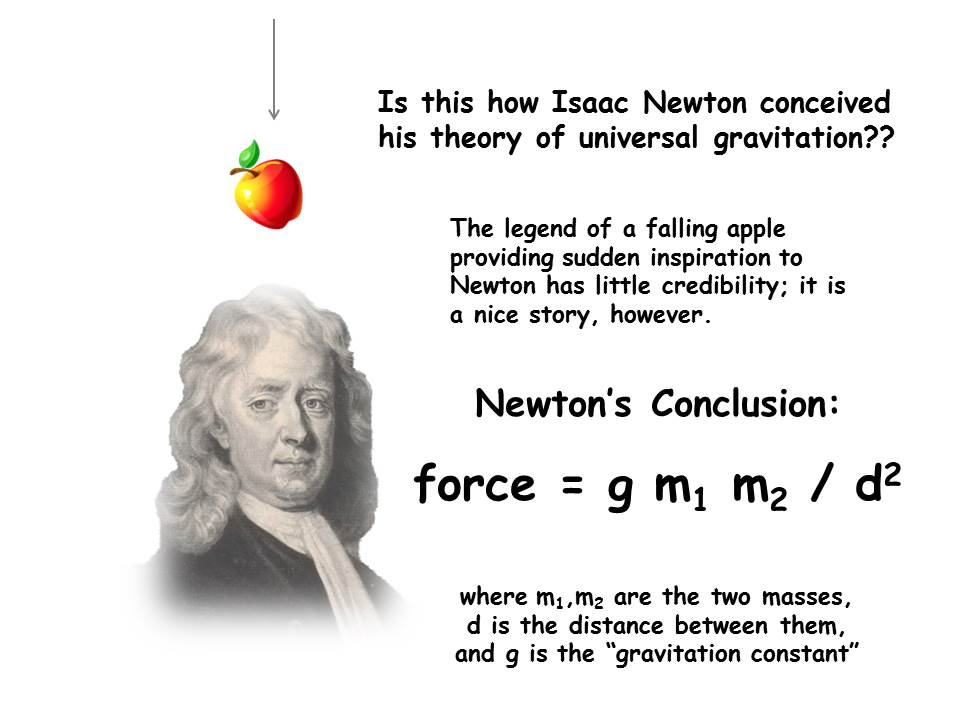
\includegraphics[width=0.6\textwidth]{fig.Newton.jpg}
  \end{figure}
https://reasonandreflection.wordpress.com/2014/02/23/the-key-to-physical-attraction-its-called-gravity-and-often-love/

\end{frame}

\begin{frame}
\frametitle{Historical Interlude}

  \begin{figure}[htb!]
    \centering
    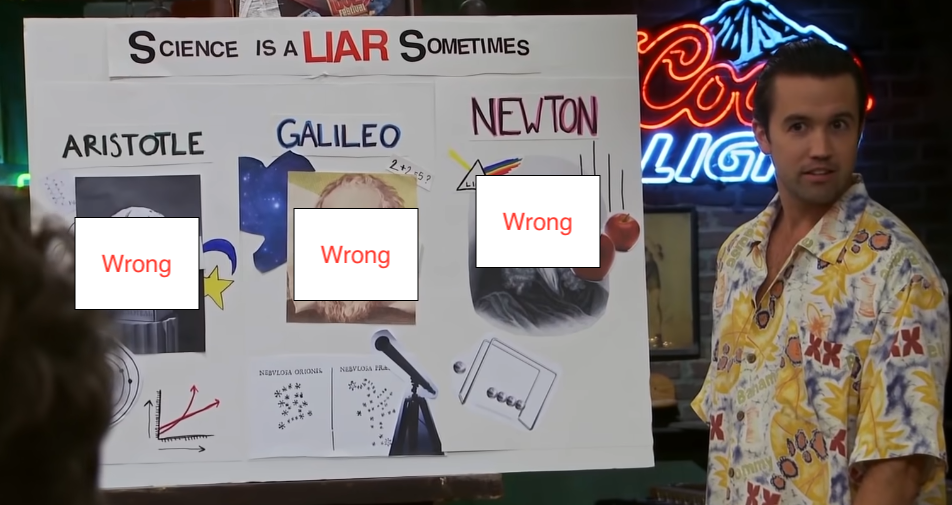
\includegraphics[width=\textwidth]{fig.macEvolution.png}
  \end{figure}

\end{frame}

\begin{frame}
\frametitle{Historical Interlude}

  \begin{figure}[htb!]
    \centering
    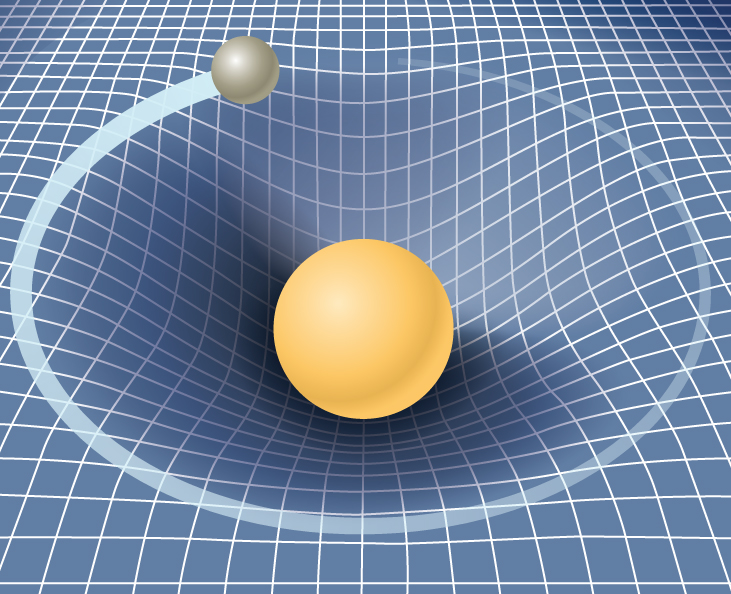
\includegraphics[width=0.6\textwidth]{fig.Einstein.jpg}
  \end{figure}
https://courses.lumenlearning.com/suny-osuniversityphysics/chapter/13-8-einsteins-theory-of-gravity/

\end{frame}

\begin{frame}
\frametitle{Importance of GR}

  \begin{figure}[htb!]
    \centering
    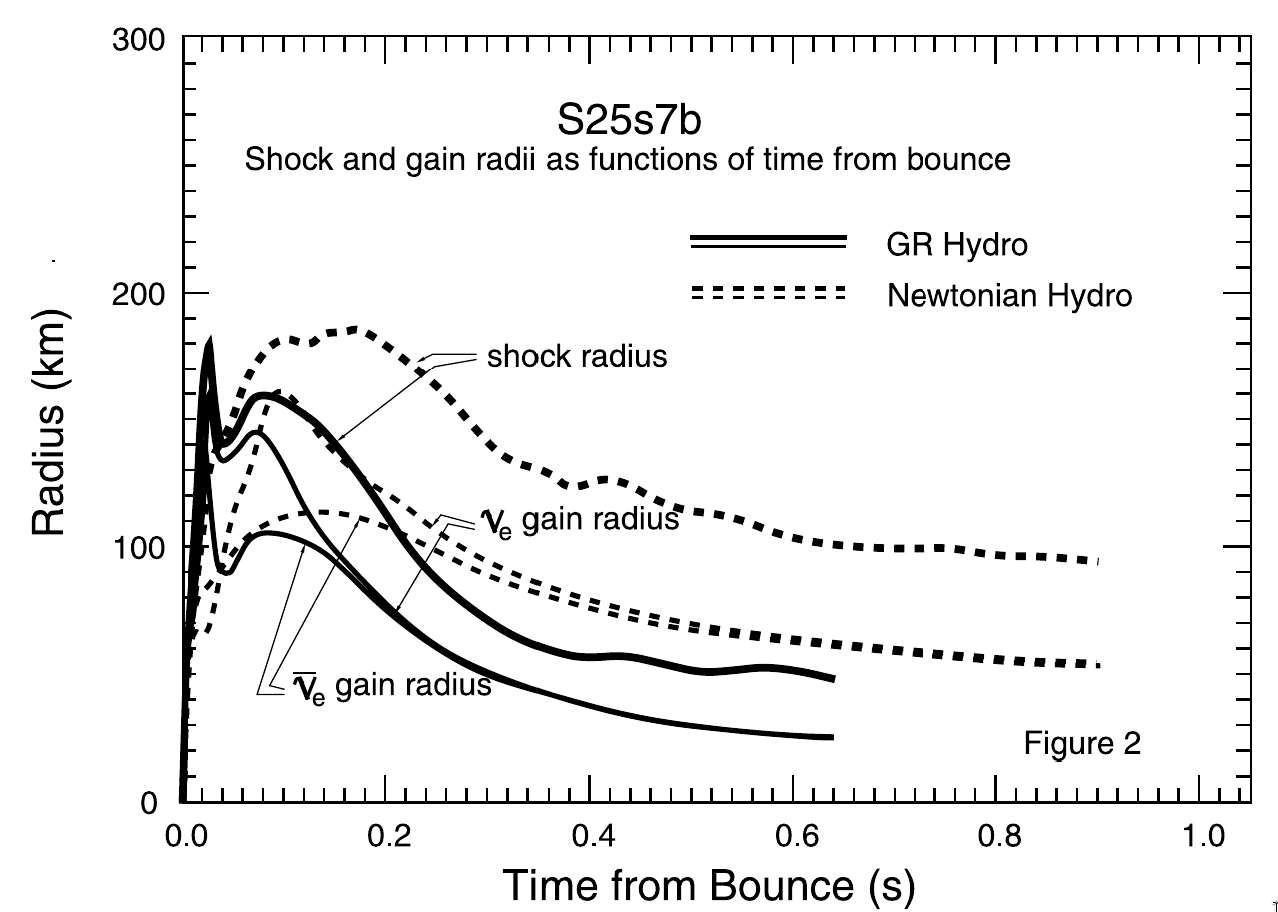
\includegraphics[width=0.7\textwidth]{fig.WhyGR.png}
  \end{figure}
  \begin{center}(Figure from \citet{lmt2001})\end{center}

\end{frame}

\begin{frame}
\frametitle{Discontinuous Galerkin (DG) Method}

  \Fontvi

  \begin{equation*}
    u\left(x\right)=1+0.1\,\sin\left(2\pi x\right)
  \end{equation*}

  \begin{figure}[htb!]
    \centering
    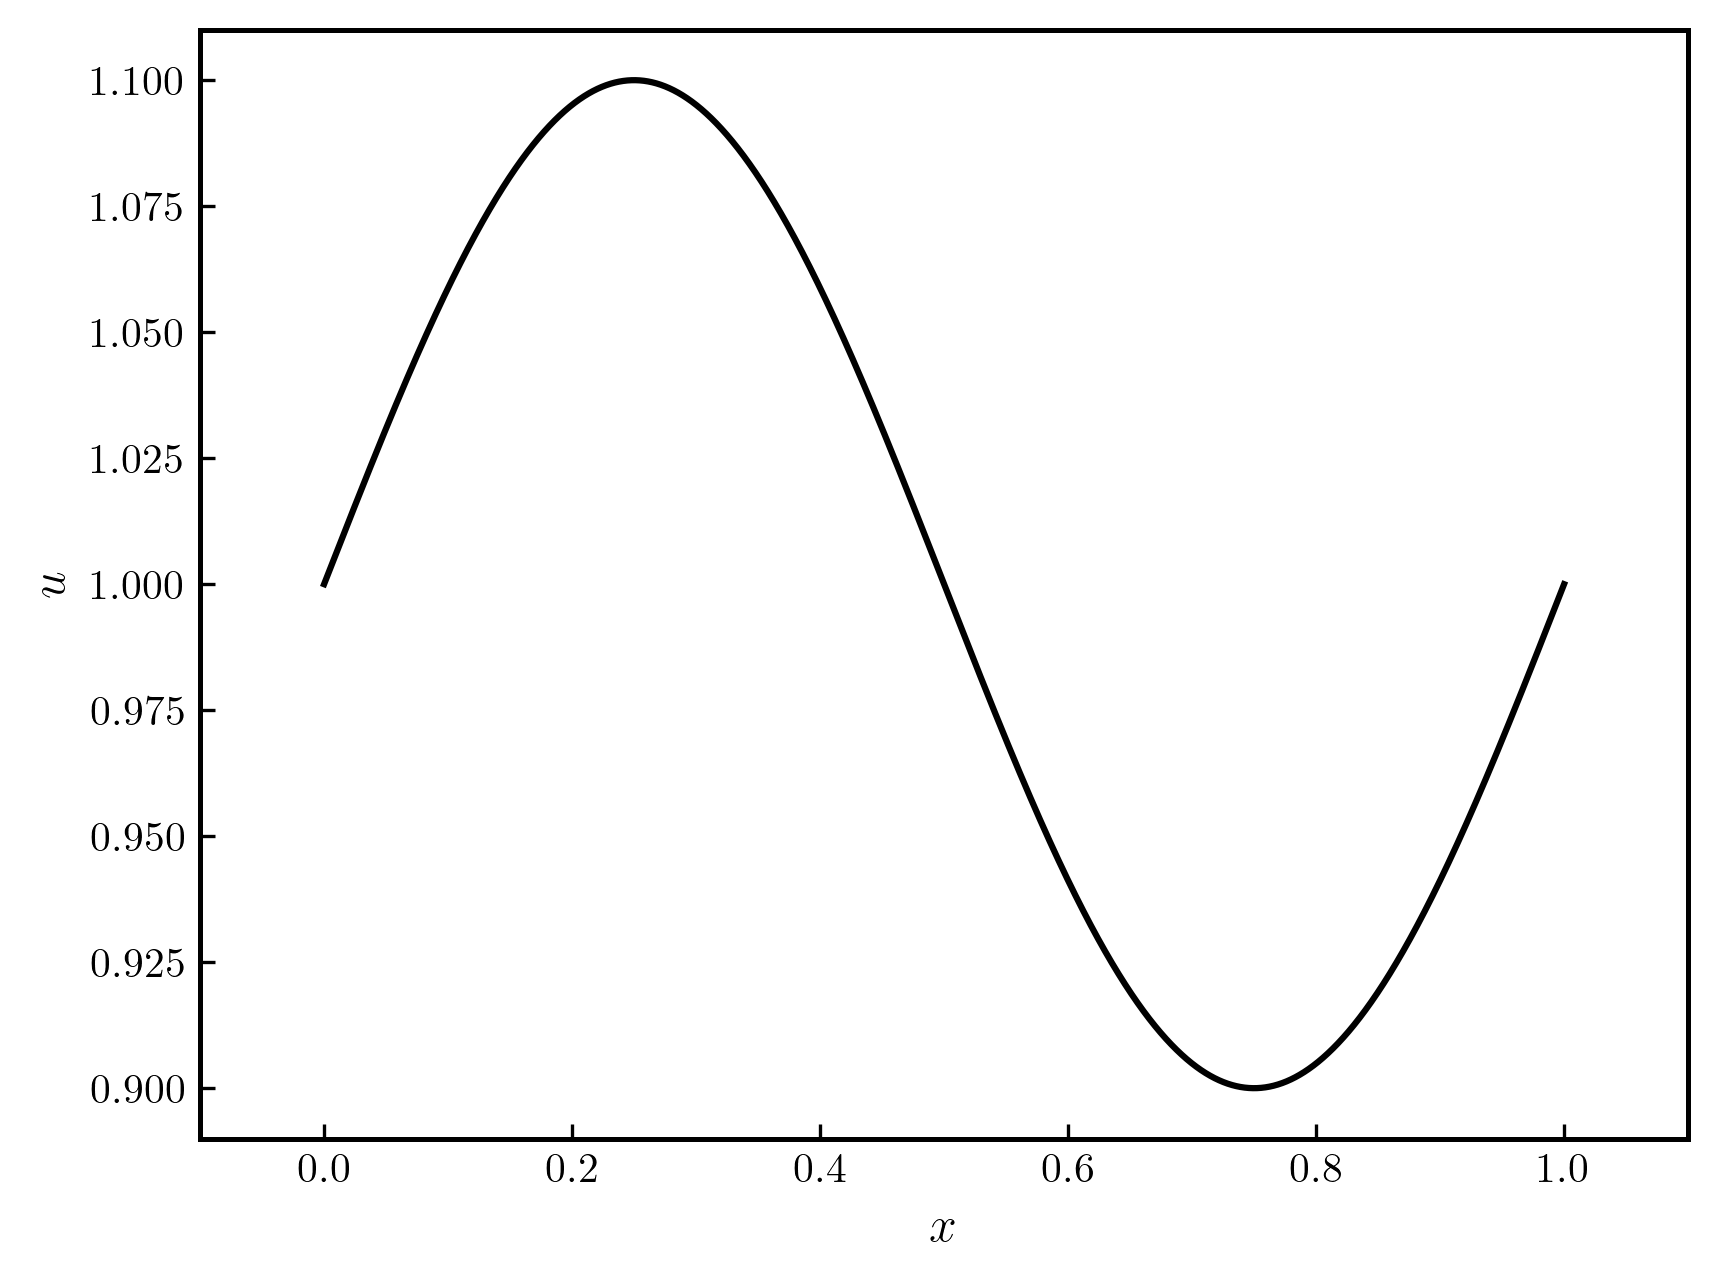
\includegraphics[width=0.7\textwidth]{fig.sine.png}
  \end{figure}

\end{frame}

\begin{frame}
\frametitle{Discontinuous Galerkin (DG) Method}

  \Fontvi

  \begin{equation*}
    u\left(x\right)=1+0.1\,\sin\left(2\pi x\right)
  \end{equation*}

  \begin{figure}[htb!]
    \centering
    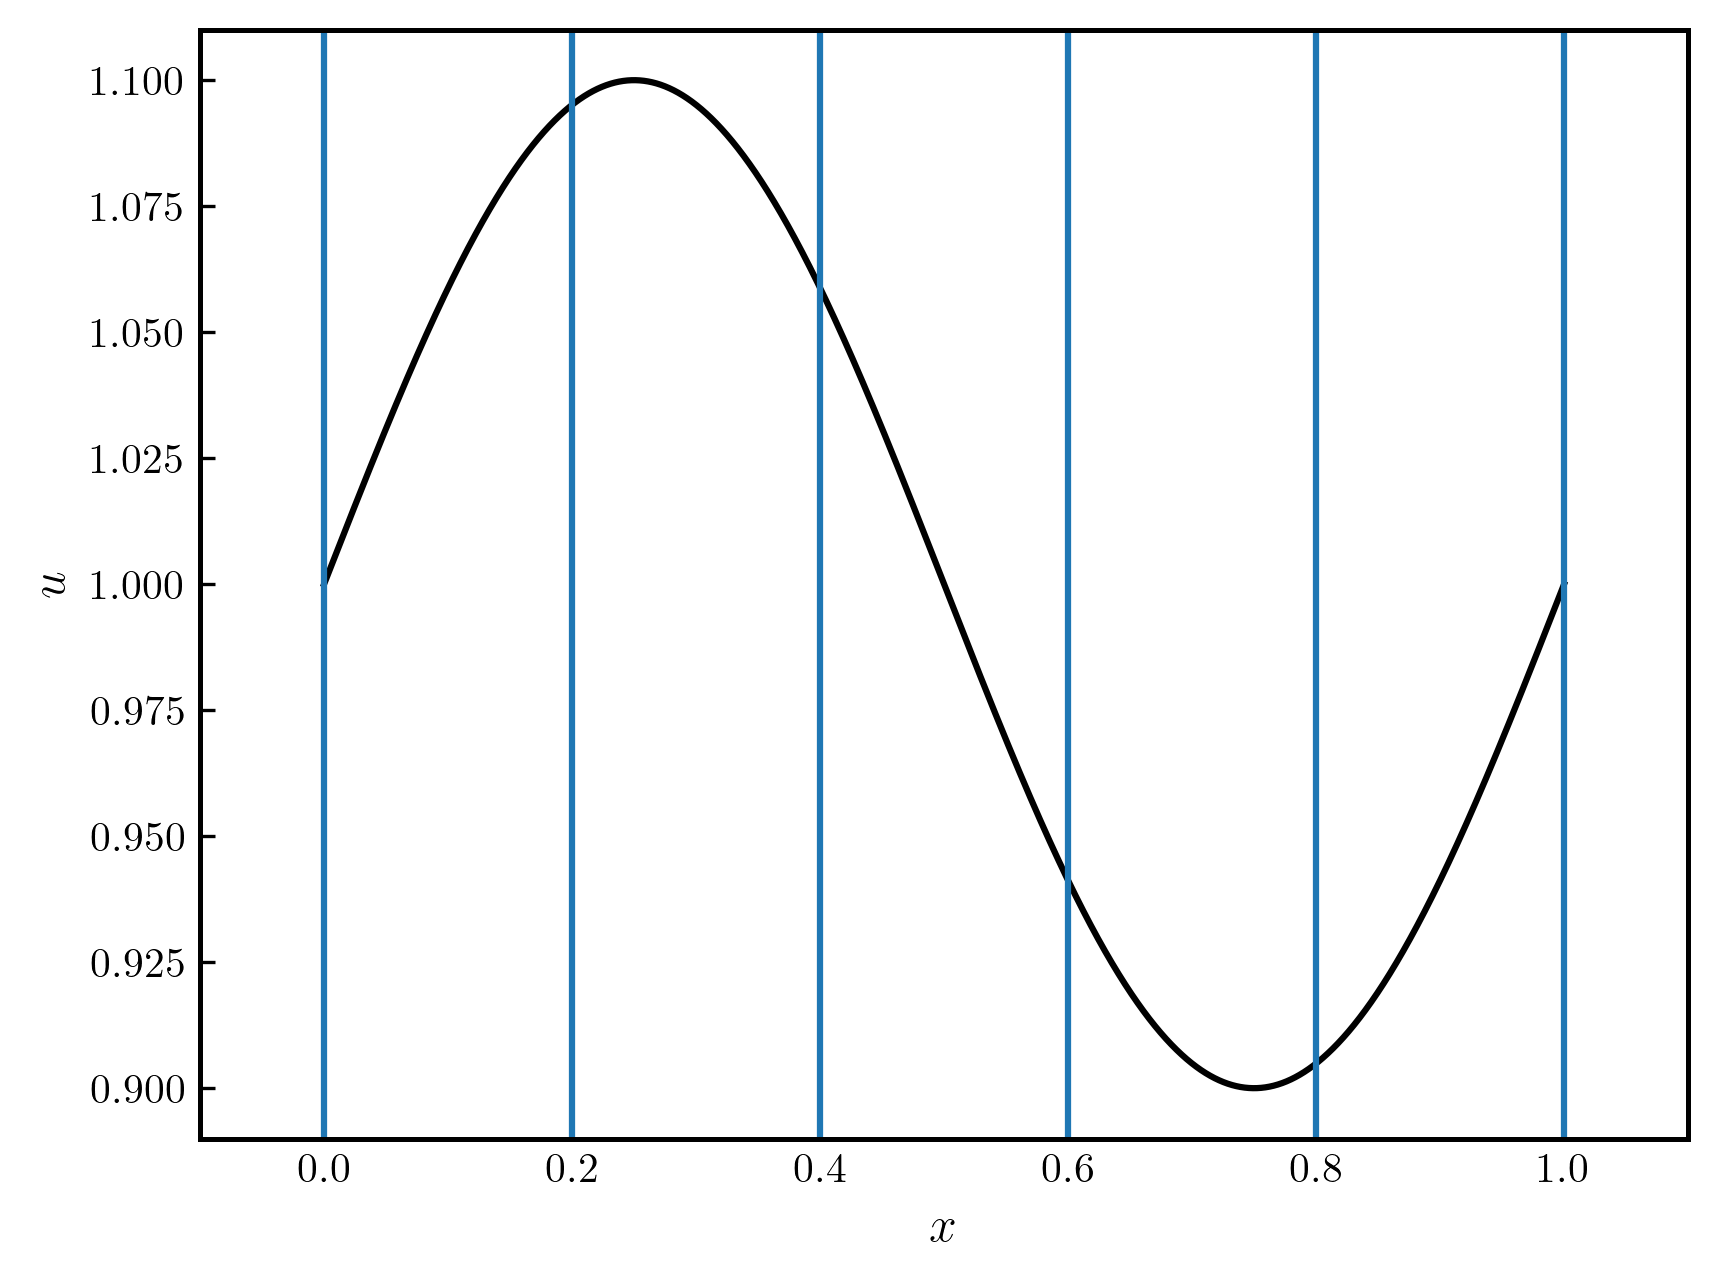
\includegraphics[width=0.7\textwidth]{fig.sineWithLines.png}
  \end{figure}

\end{frame}

\begin{frame}
\frametitle{Discontinuous Galerkin (DG) Method}

  \Fontvi

  \begin{equation*}
    u\left(x\right)=1+0.1\,\sin\left(2\pi x\right)
  \end{equation*}

  \begin{figure}[htb!]
    \centering
    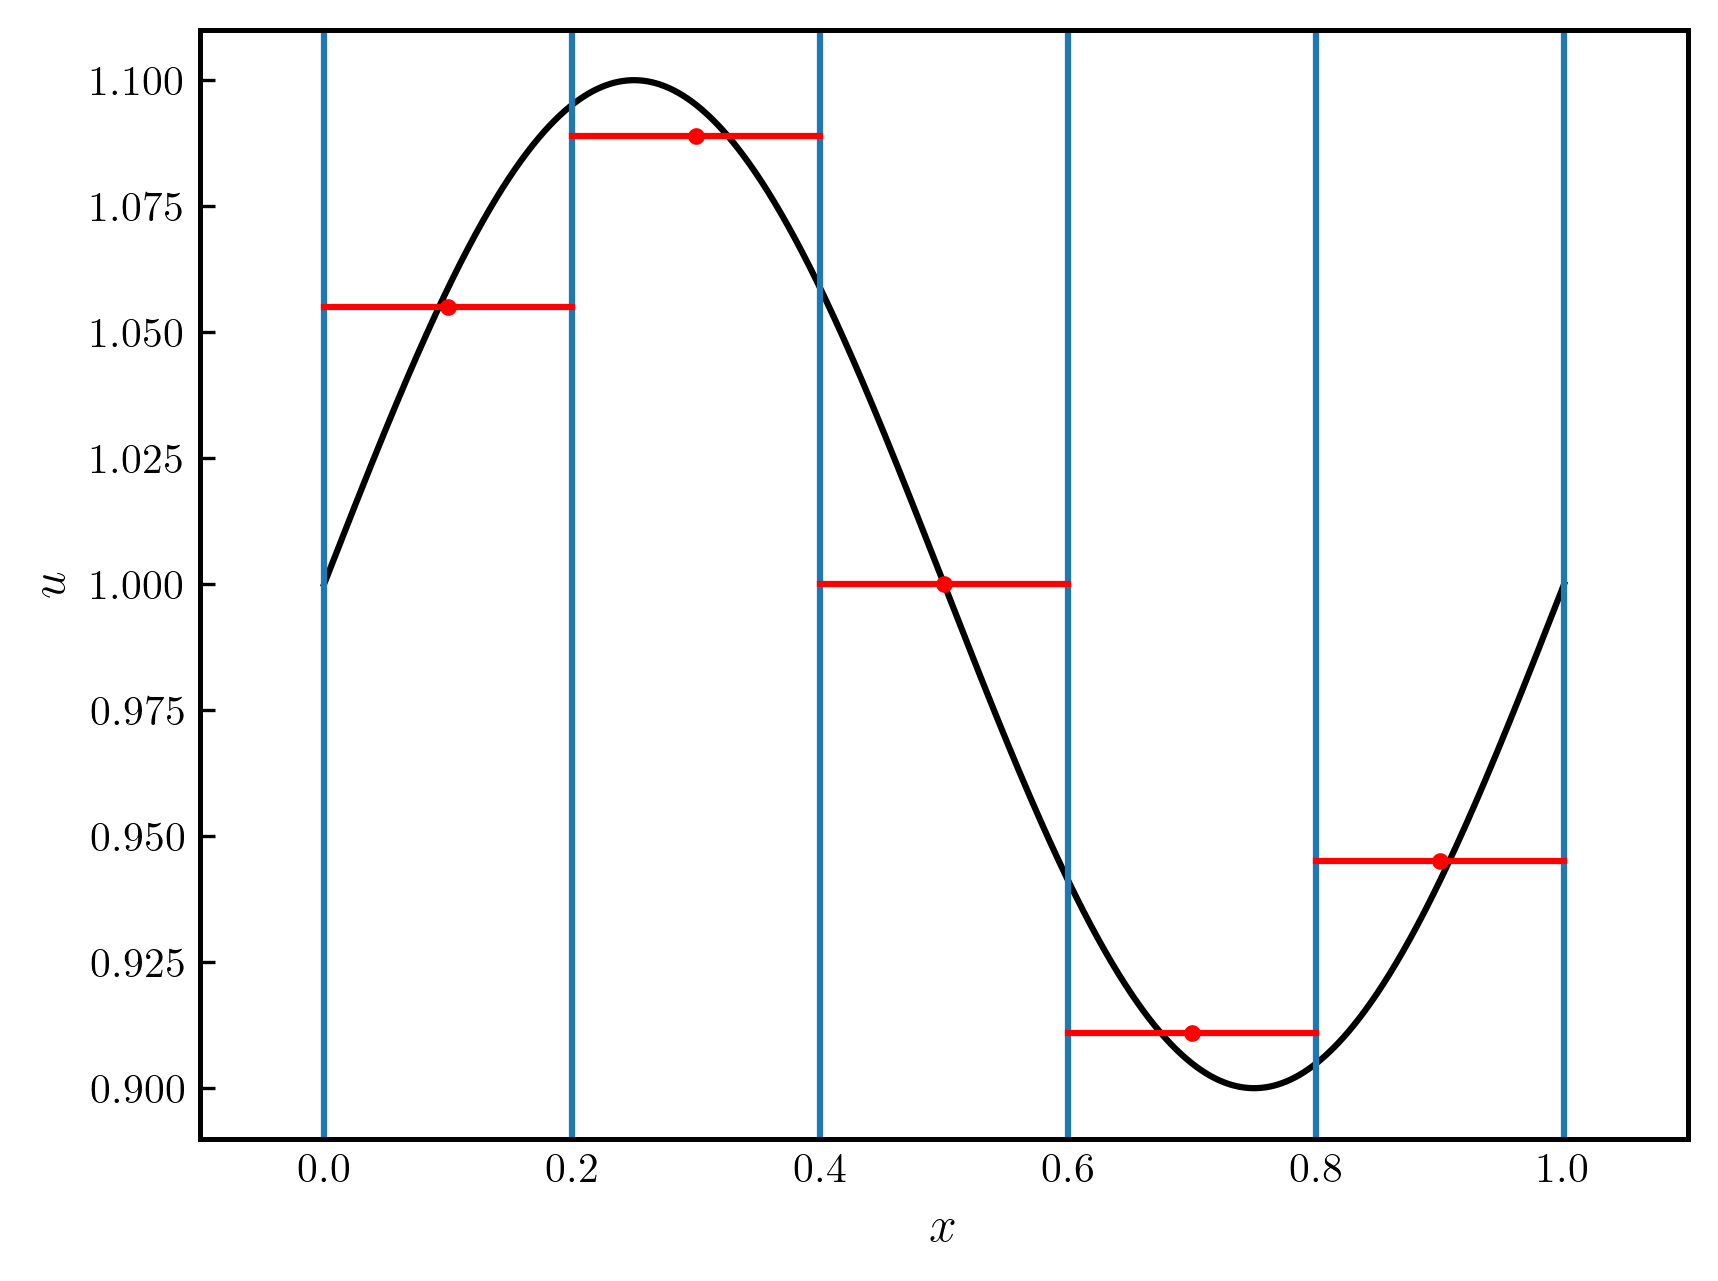
\includegraphics[width=0.7\textwidth]{fig.sineWithLines_DG0.png}
  \end{figure}

\end{frame}

\begin{frame}
\frametitle{Discontinuous Galerkin (DG) Method}

  \Fontvi

  \begin{equation*}
    u\left(x\right)=1+0.1\,\sin\left(2\pi x\right)
  \end{equation*}

  \begin{figure}[htb!]
    \centering
    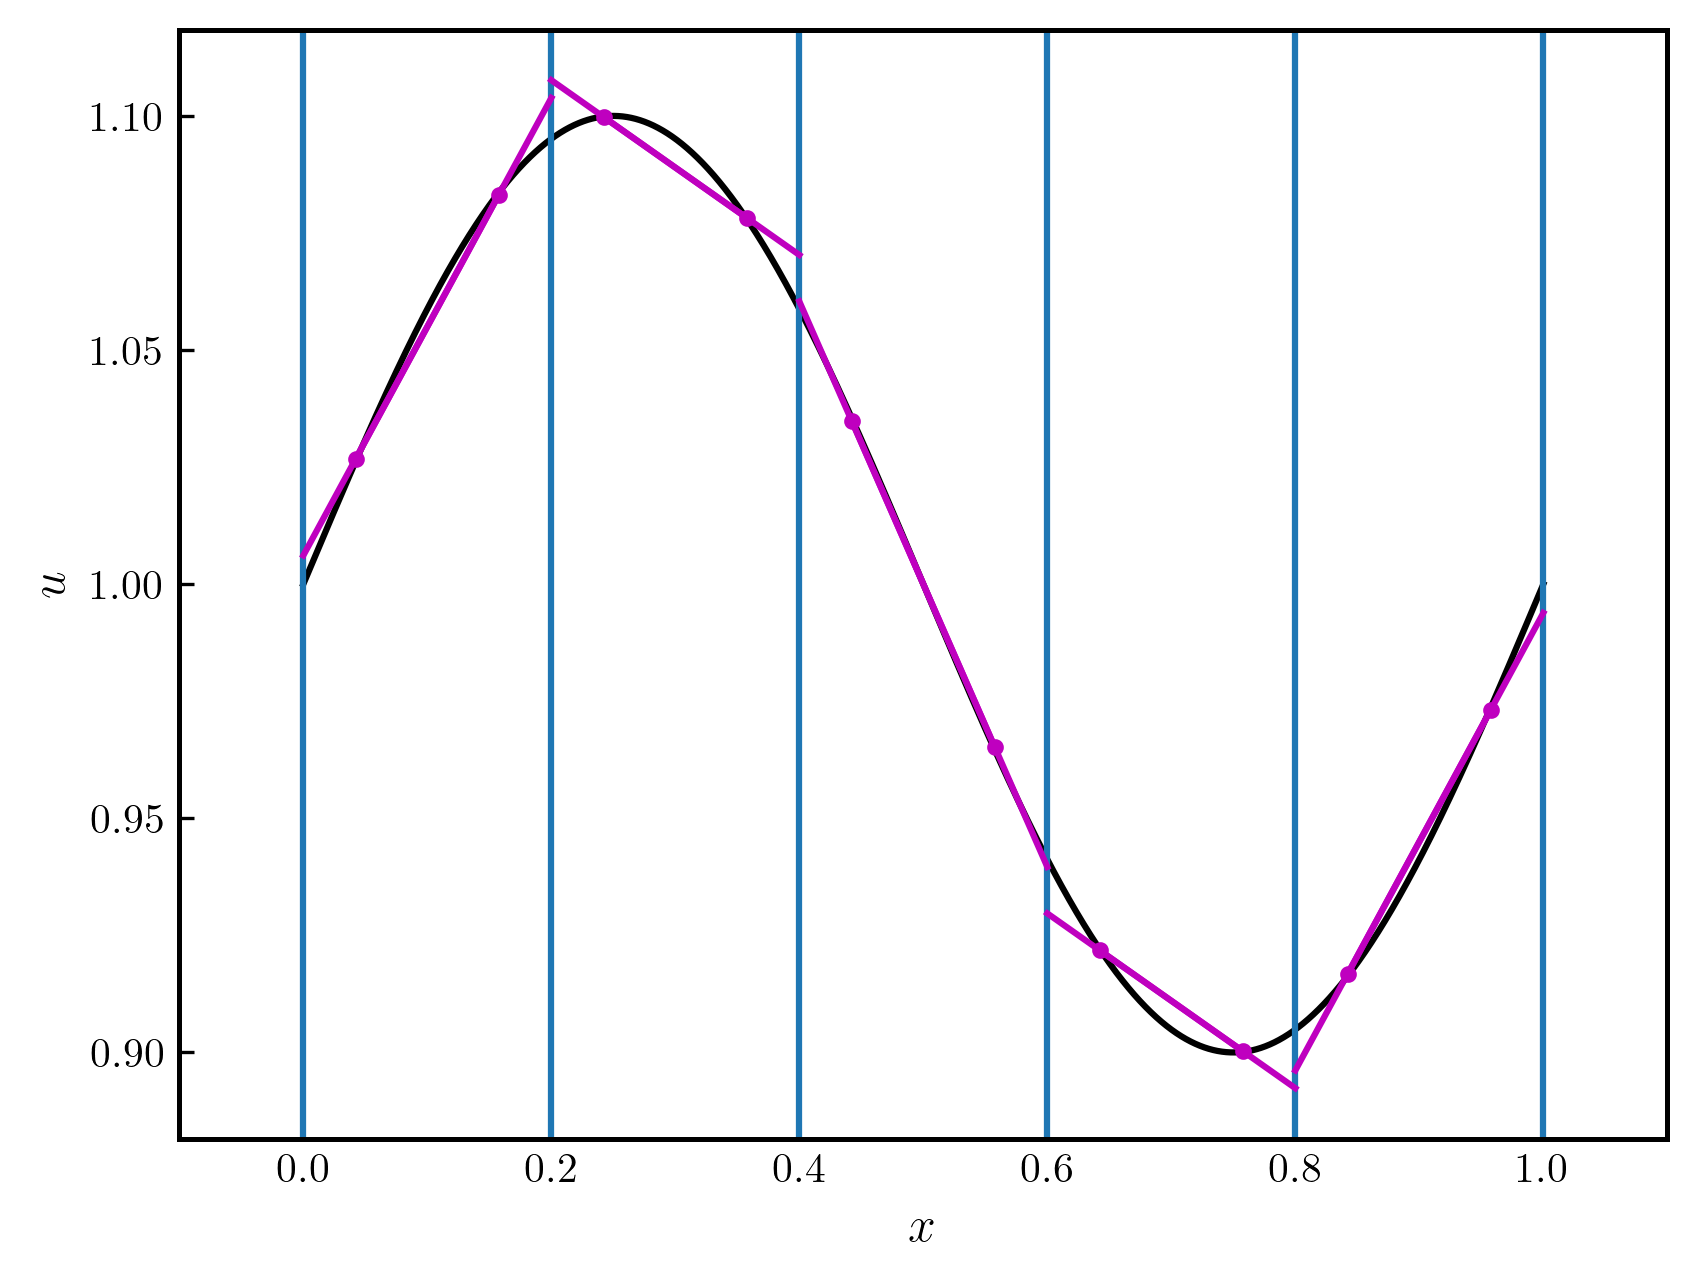
\includegraphics[width=0.7\textwidth]{fig.sineWithLines_DG1.png}
  \end{figure}

\end{frame}

\begin{frame}
\frametitle{Discontinuous Galerkin (DG) Method}

  \Fontvi

  \begin{equation*}
    u\left(x\right)=1+0.1\,\sin\left(2\pi x\right)
  \end{equation*}

  \begin{figure}[htb!]
    \centering
    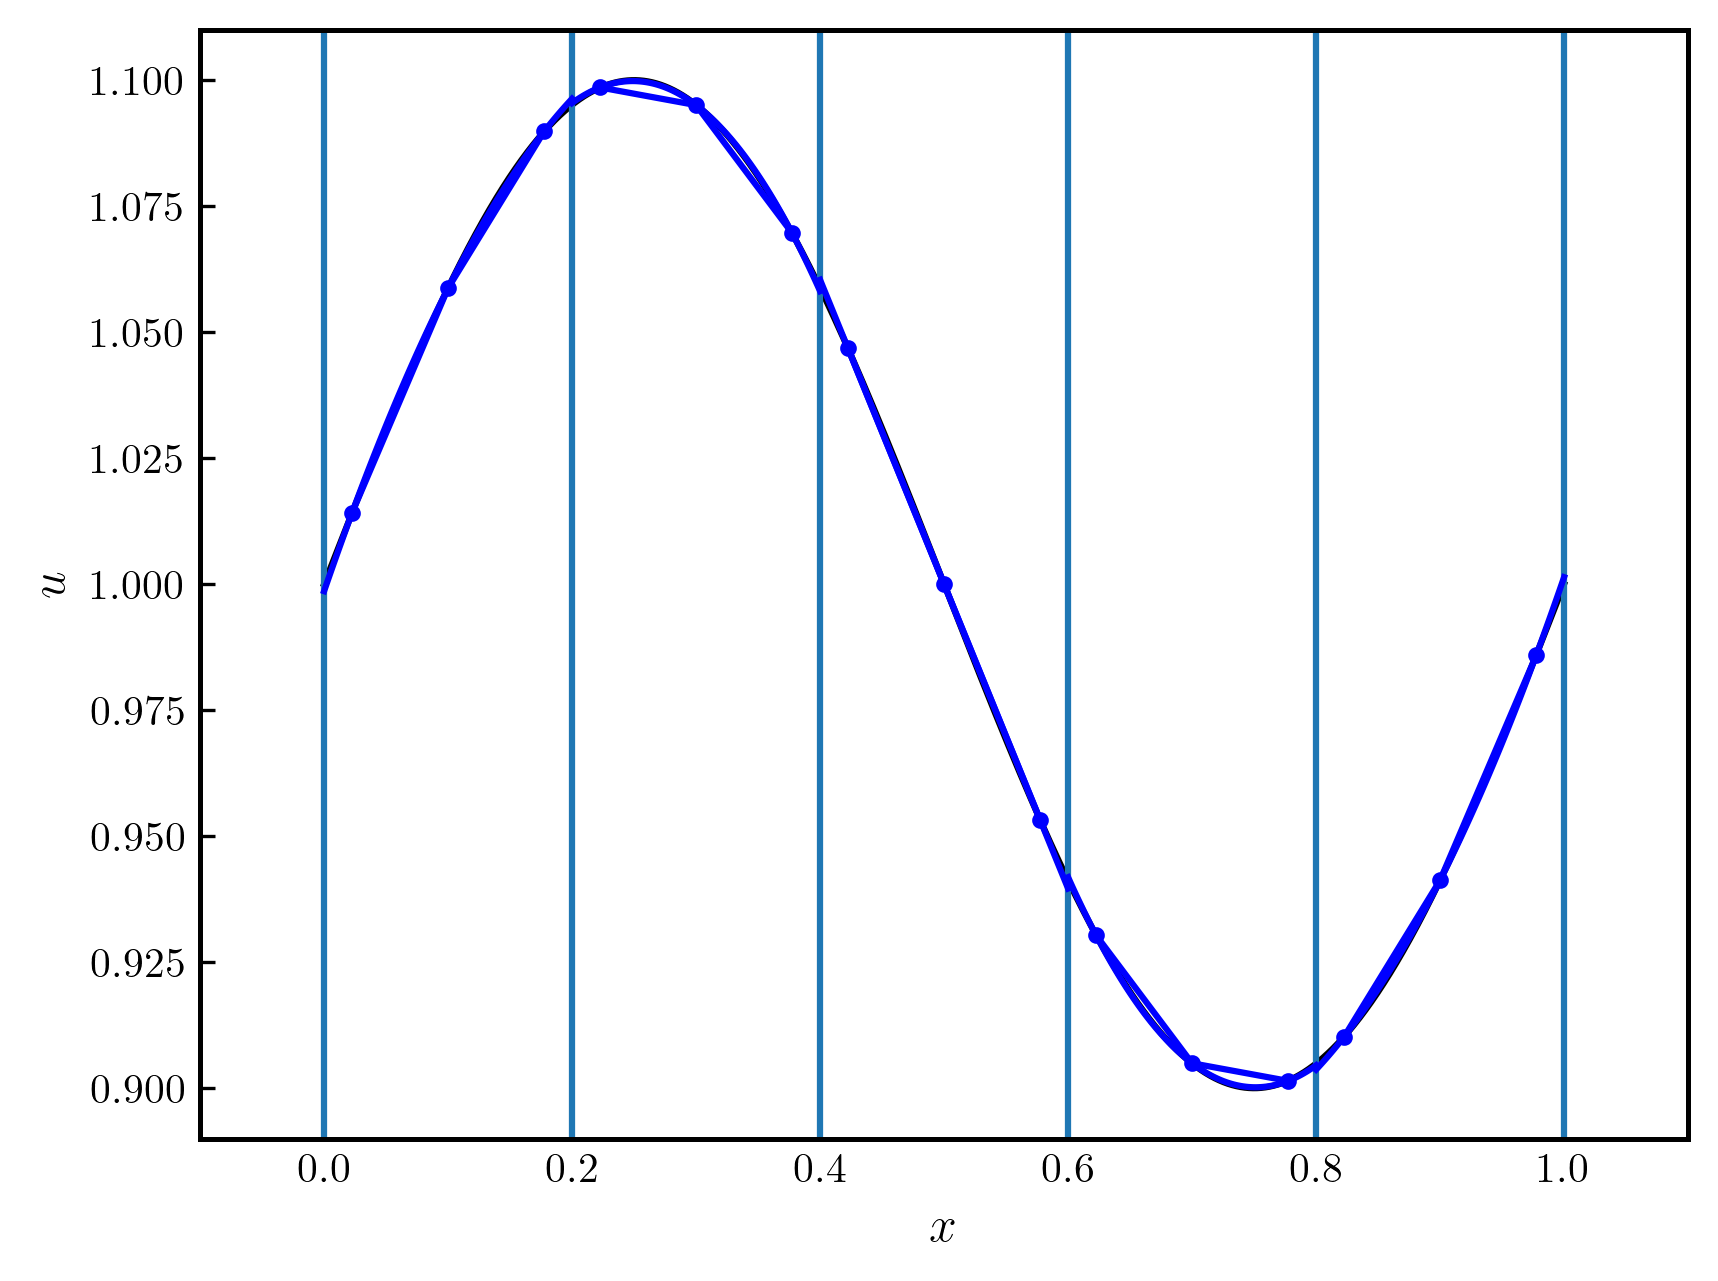
\includegraphics[width=0.7\textwidth]{fig.sineWithLines_DG2.png}
  \end{figure}

\end{frame}

\begin{frame}
\frametitle{Discontinuous Galerkin (DG) Method}

  \Fontvi

  \begin{equation*}
    u_{h}\left(x,t\right)
    :=\sum\limits_{i=1}^{N}
      u_{i}\left(t\right)\,\ell_{i}\left(x\right)
  \end{equation*}

  \begin{figure}[htb!]
    \centering
    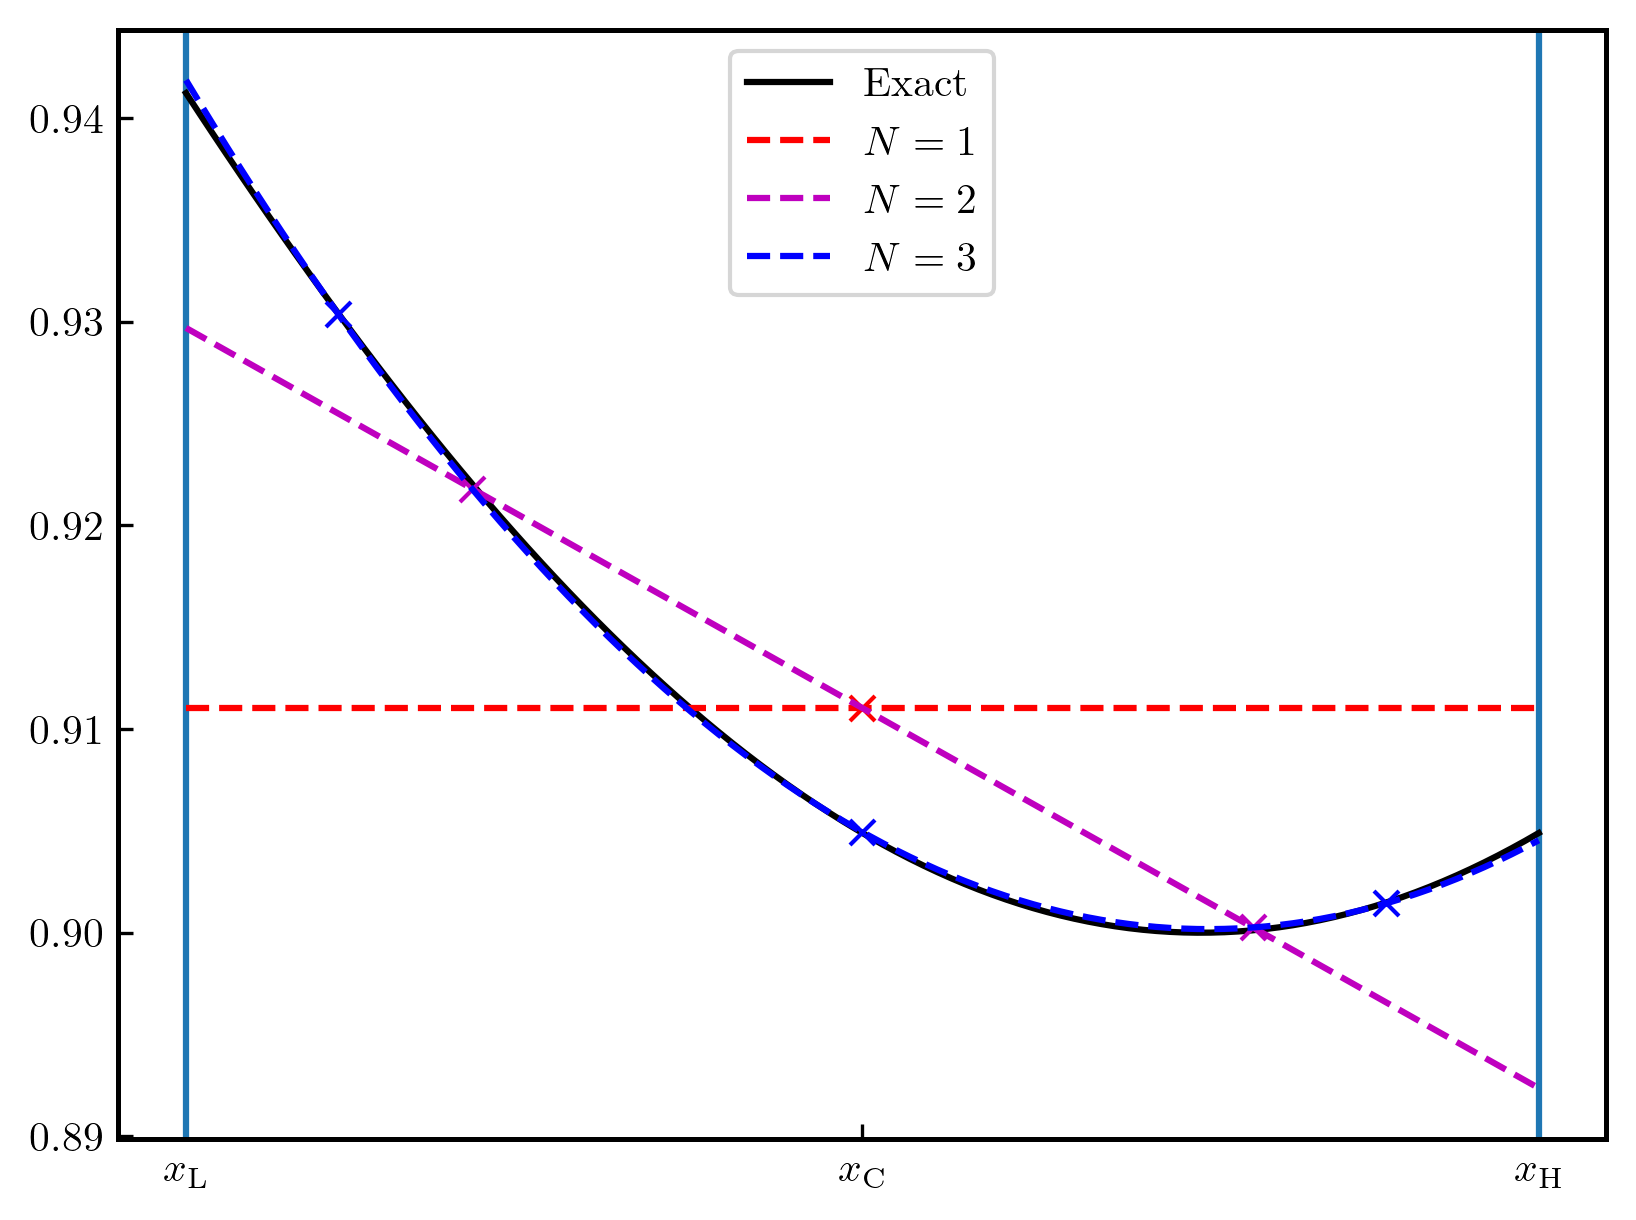
\includegraphics[width=0.7\textwidth]{fig.DG_1D.png}
  \end{figure}

\end{frame}

\begin{frame}

  \begin{figure}[htb!]
    \centering
    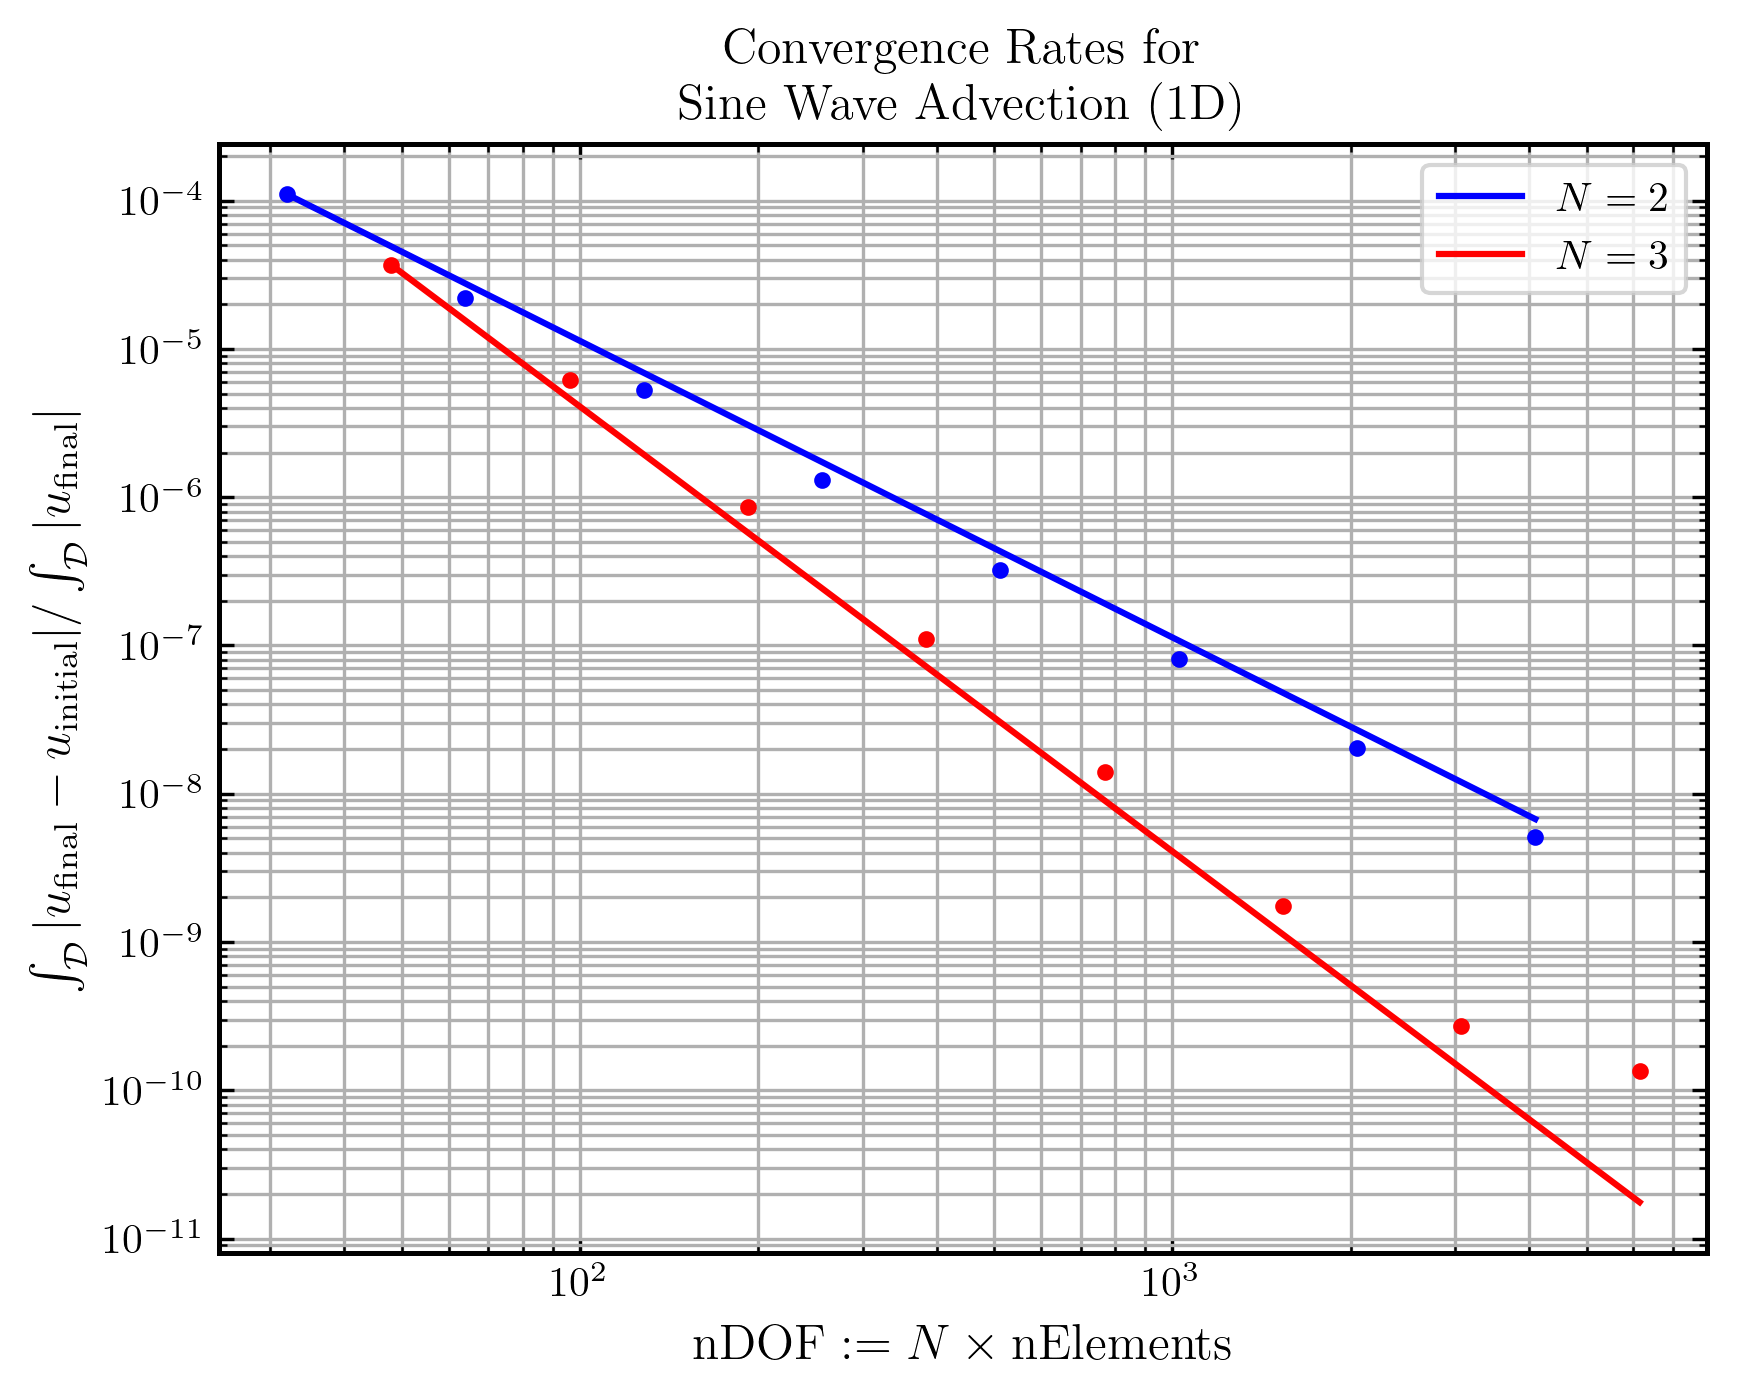
\includegraphics[width=0.8\textwidth]{fig.ConvergenceRates.png}
  \end{figure}

\end{frame}

\begin{frame}
\frametitle{Standing Accretion Shock Instability}

  Used \thornado{} to investigate the role of GR on the SASI%
  \footnote{\citet{dem2020,dem2023}}

  \begin{columns}[c]

    \column{.6\textwidth}

      \begin{figure}[htb!]
        \centering
        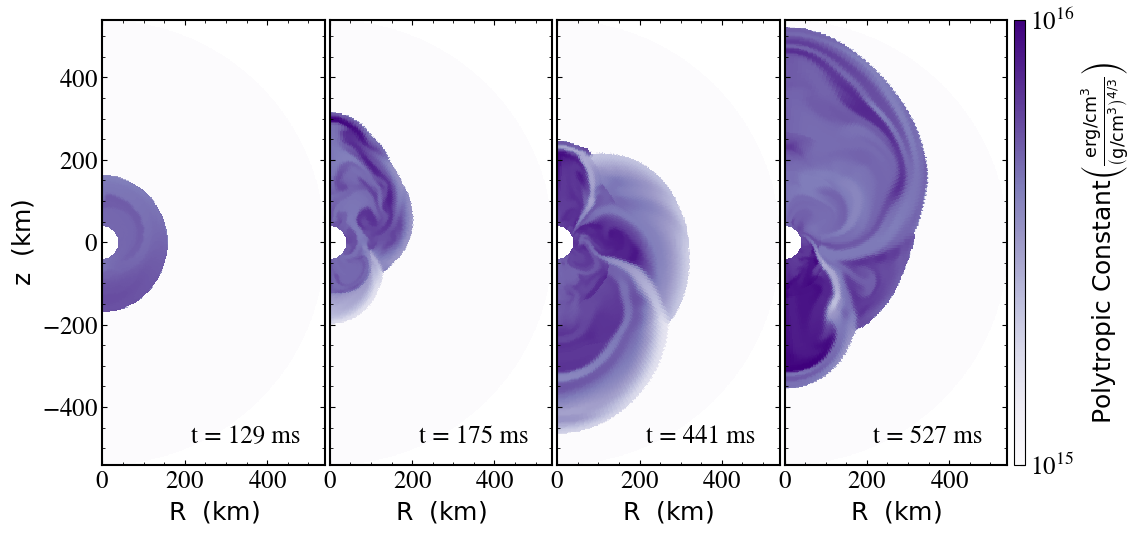
\includegraphics[width=0.9\textwidth]{fig.sasi.png}
      \end{figure}

    \column{.4\textwidth}

      \begin{figure}[htb!]
        \centering
        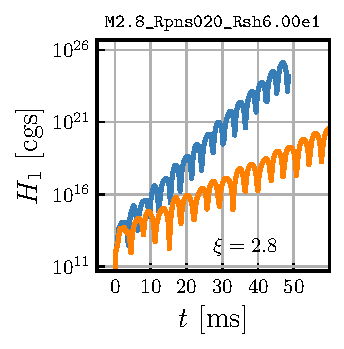
\includegraphics[width=0.9\textwidth]{fig.sasi_GRvNR.pdf}
      \end{figure}

  \end{columns}

\end{frame}

\begin{frame}
\frametitle{Mesh Refinement}

  \begin{figure}[htb!]
    \centering
    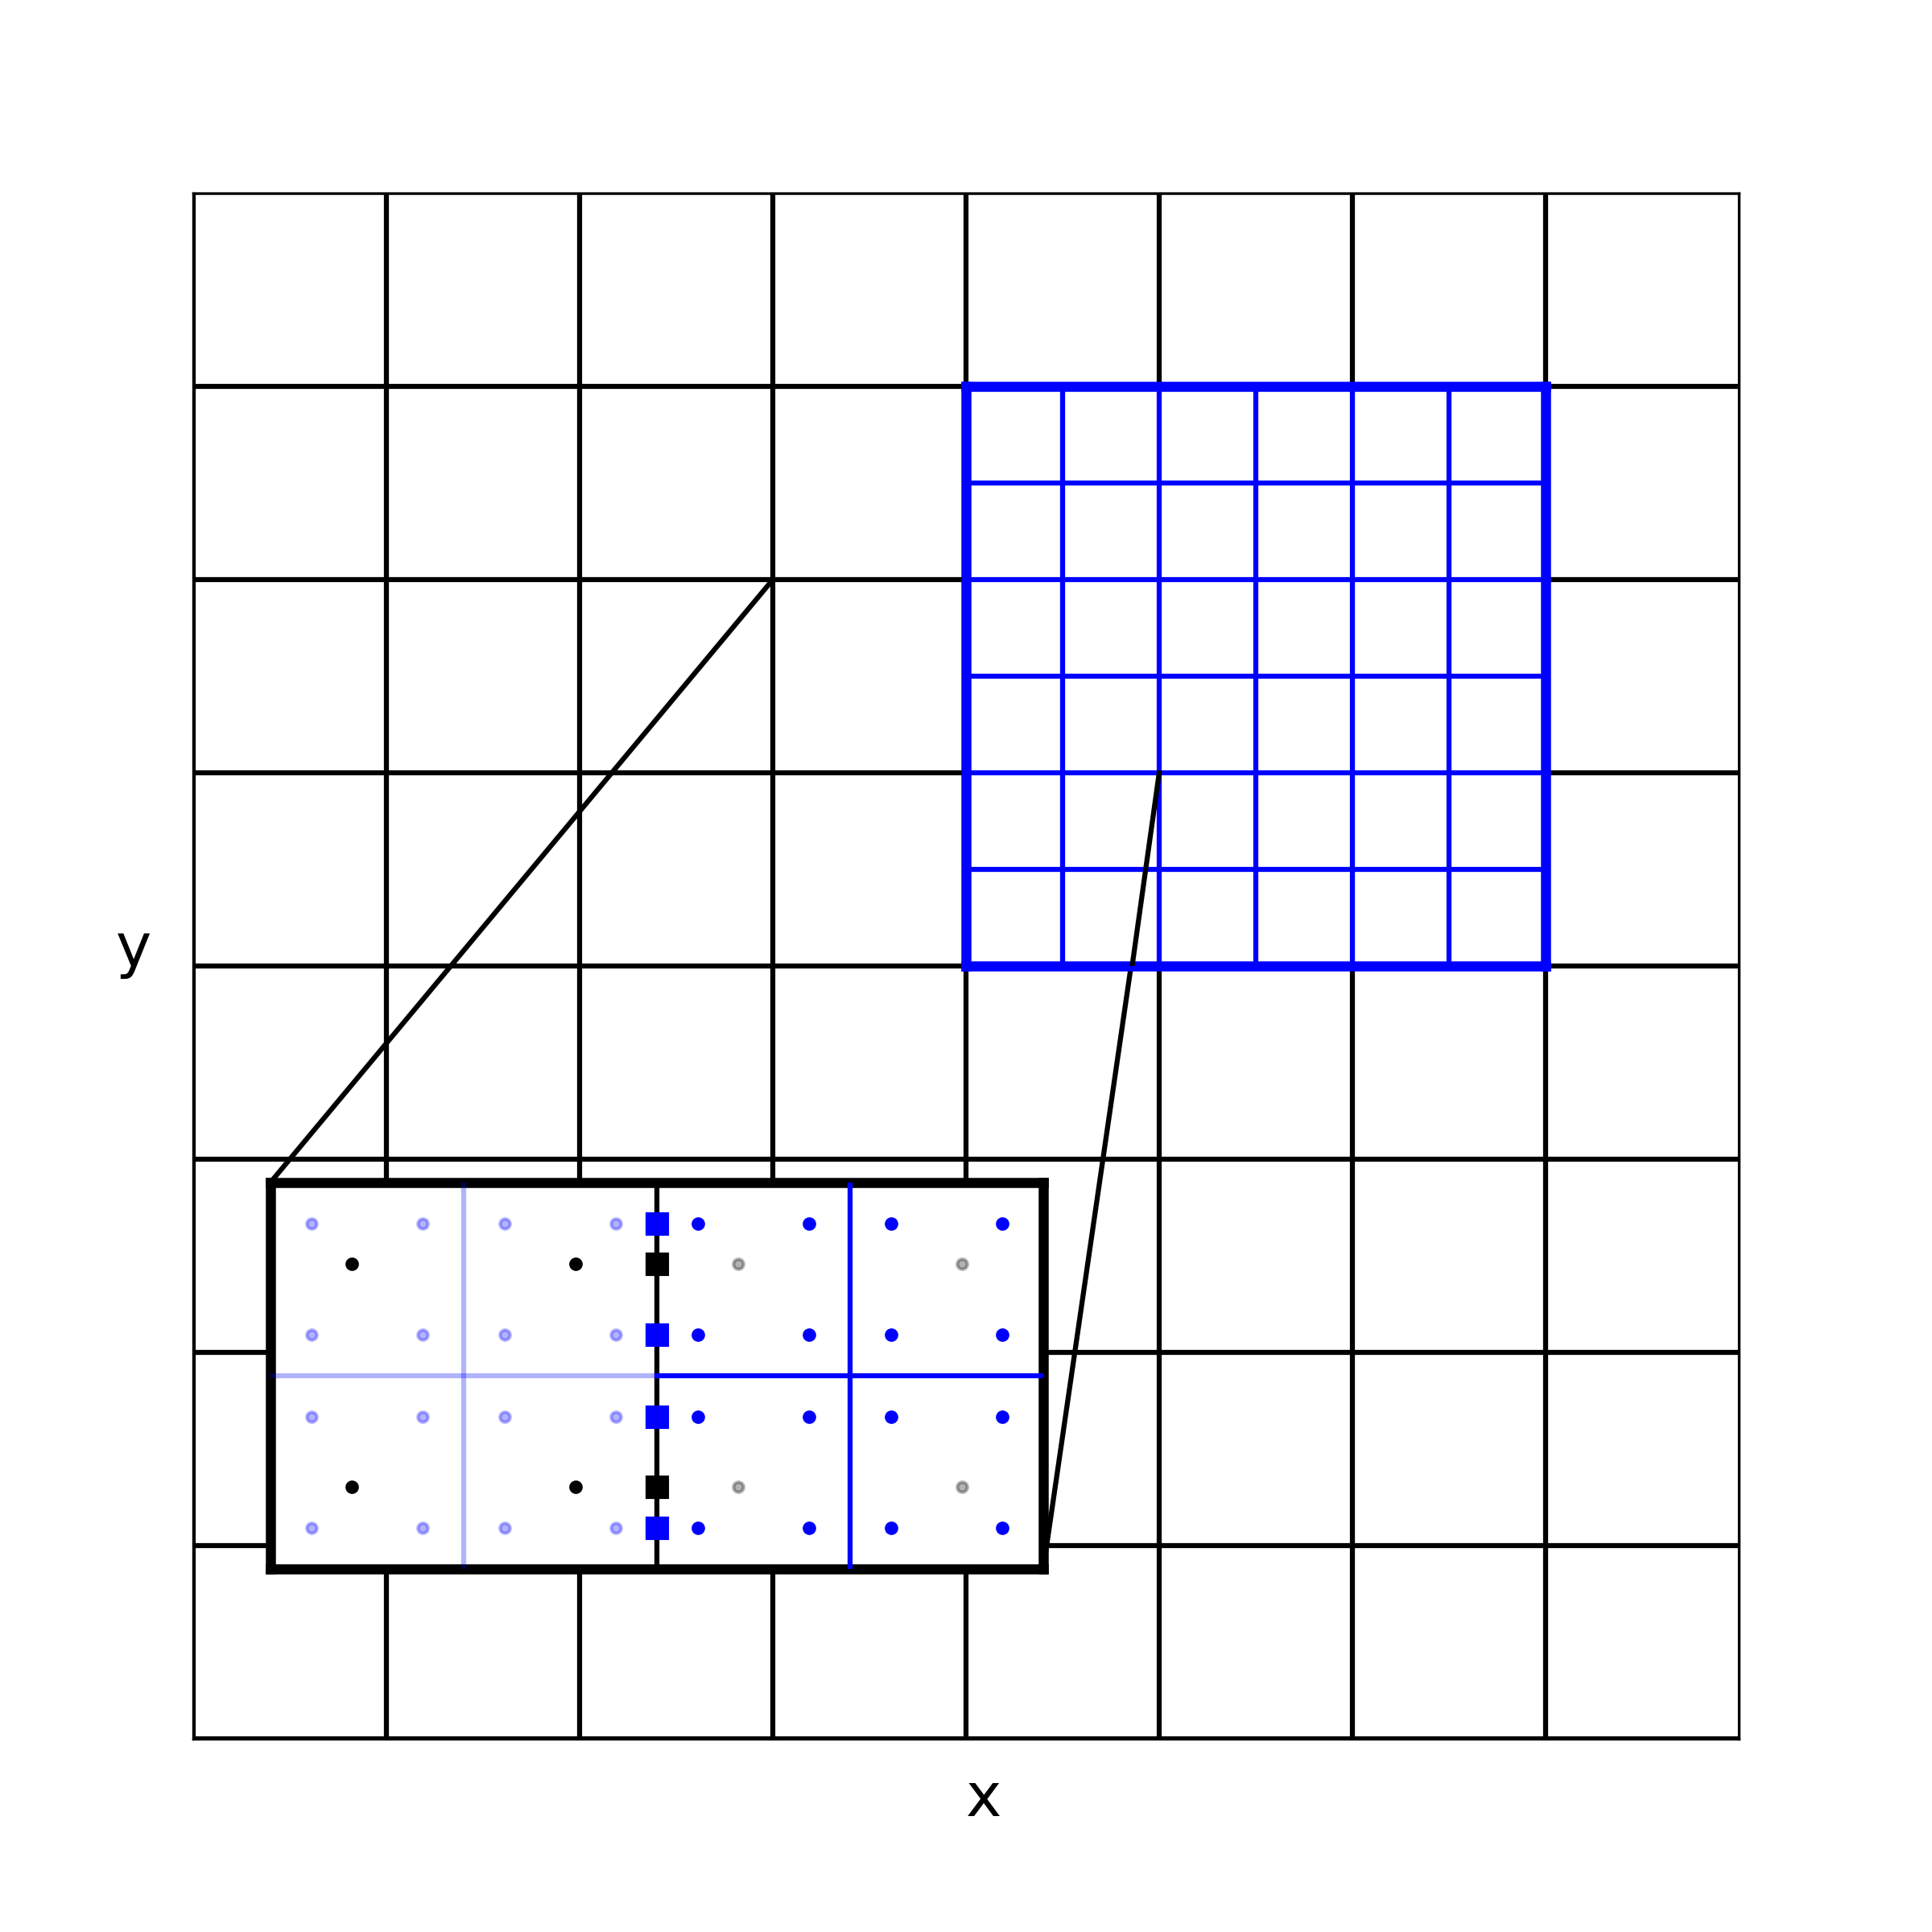
\includegraphics[width=0.7\textwidth]{fig.MeshRefinement_2D.png}
  \end{figure}

\end{frame}

\begin{frame}
\frametitle{Kelvin--Helmholtz Instability}

  \begin{center}
    {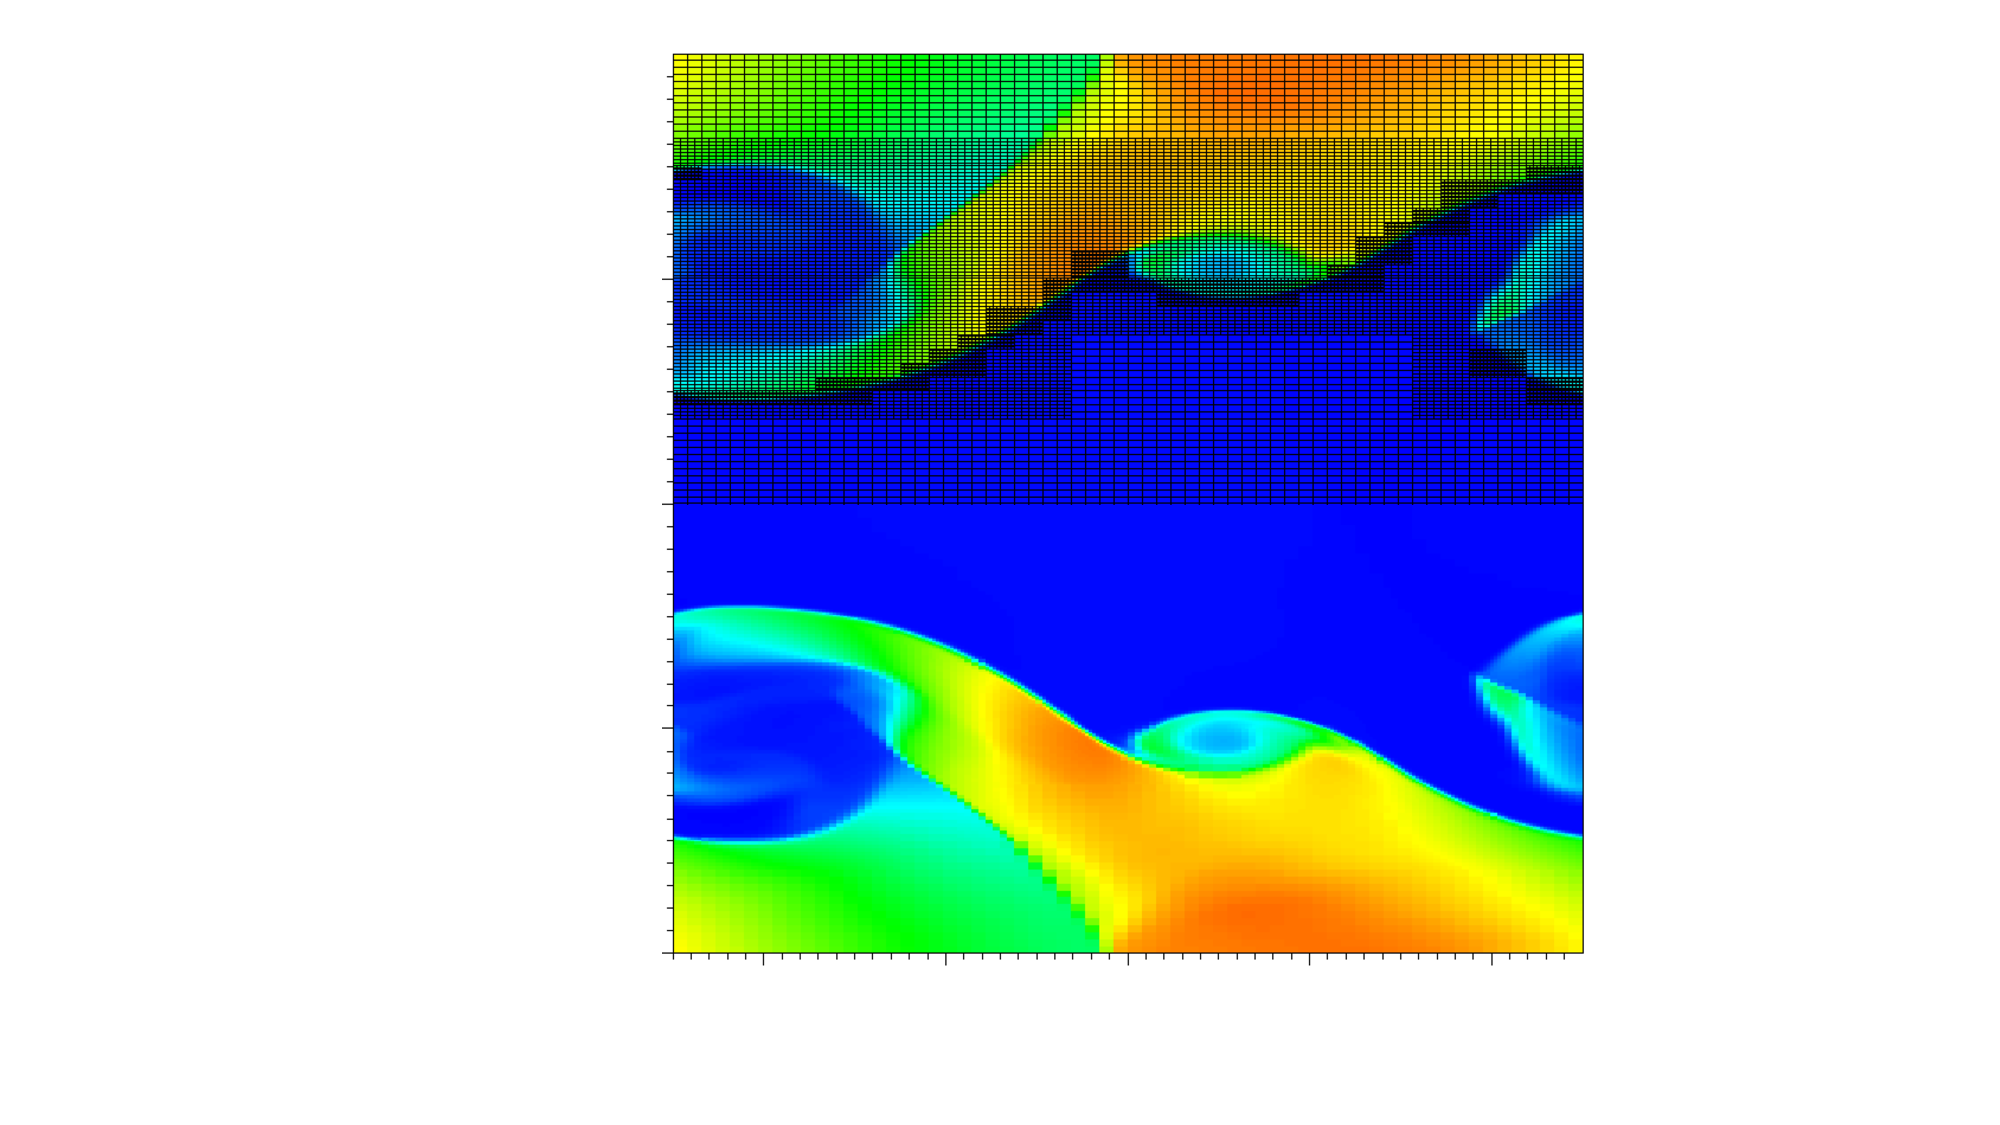
\includegraphics[width=0.6\textwidth]{fig.KHI.pdf}}
  \end{center}

\end{frame}

\begin{frame}
\frametitle{Adiabatic Collapse (AMR, Collapse Phase)}

  \begin{figure}[htb!]
    \centering
    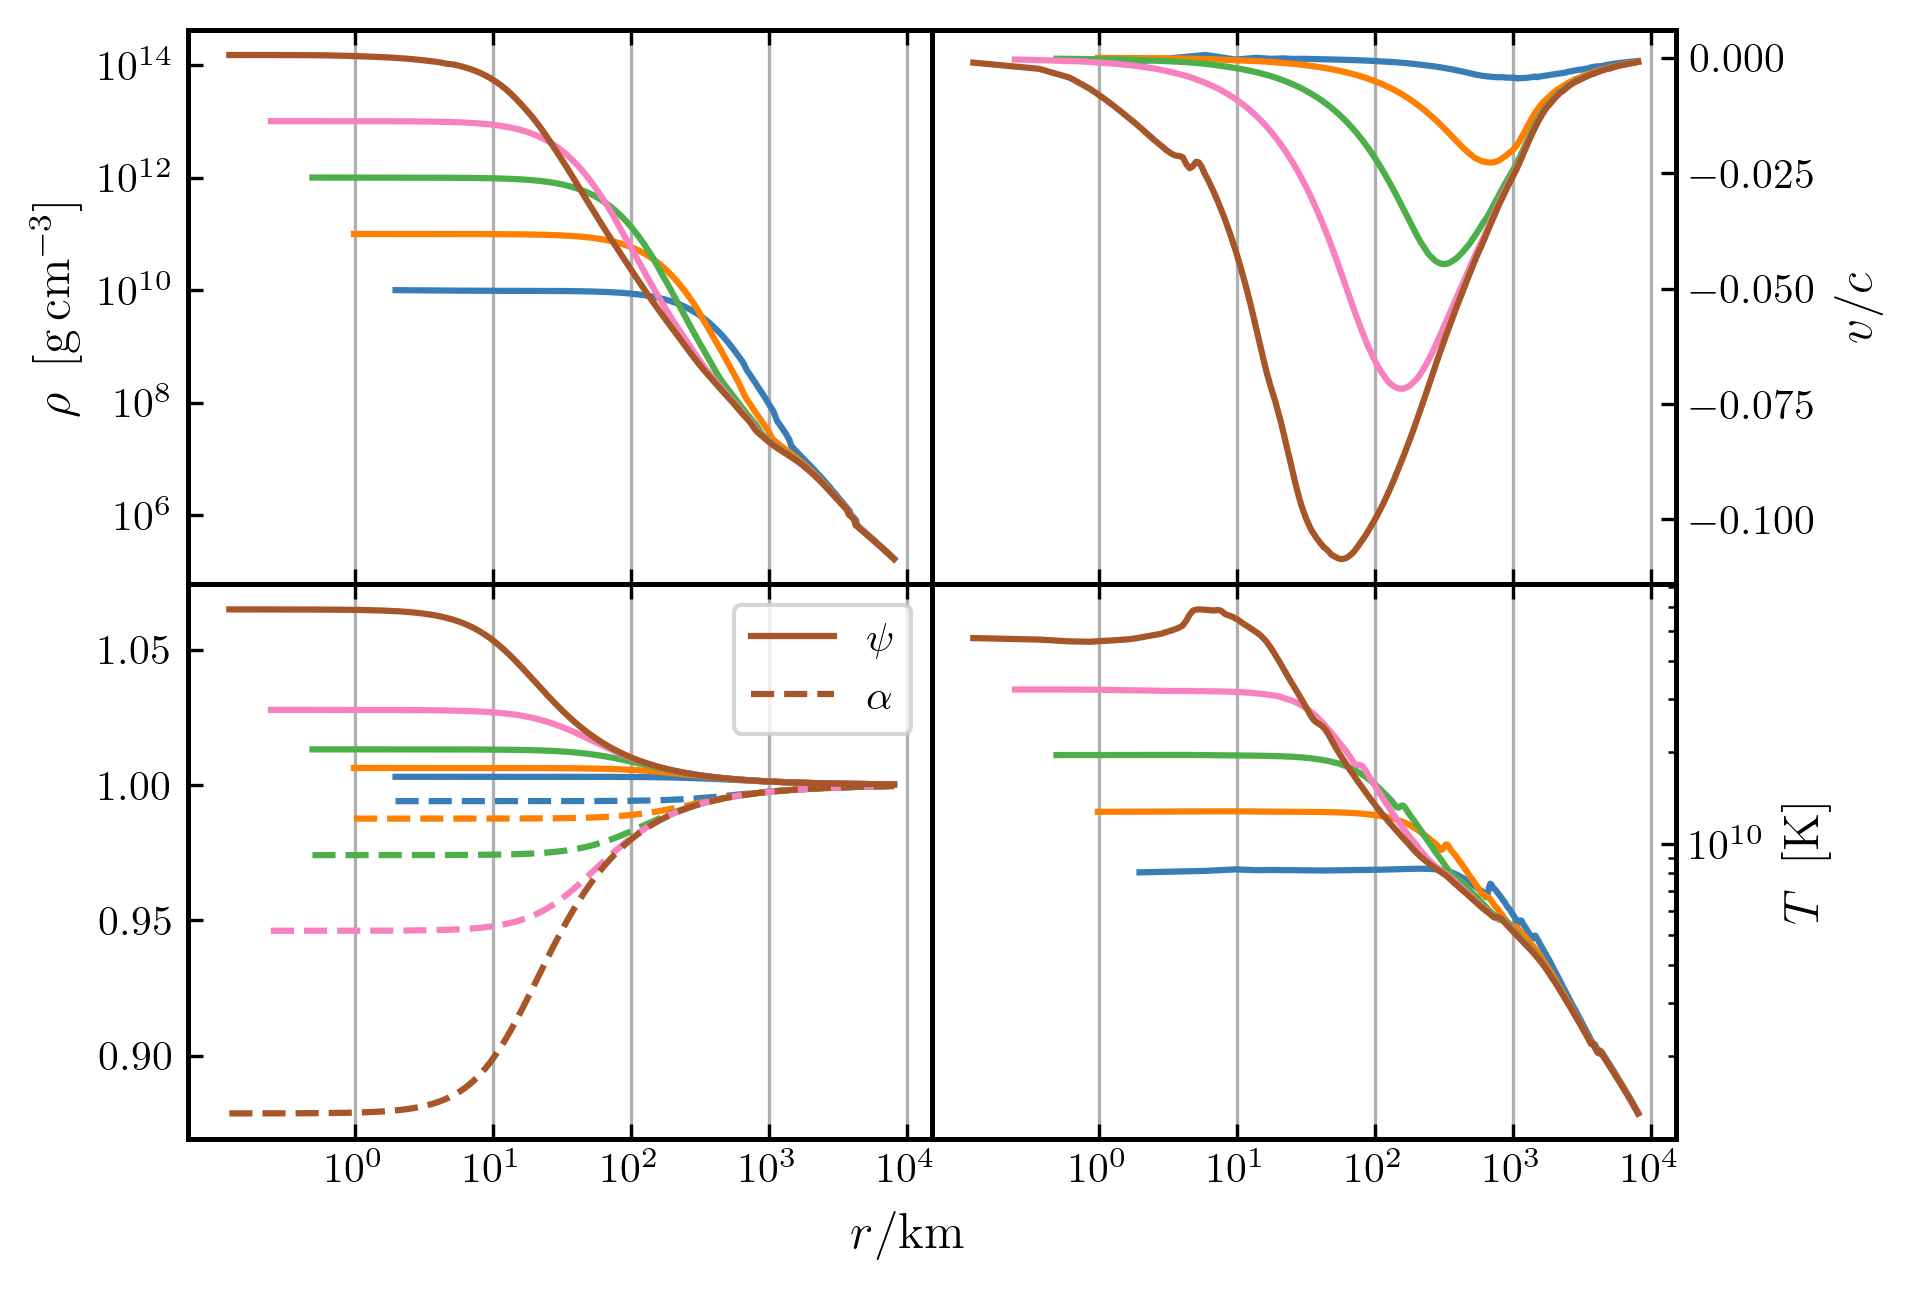
\includegraphics[width=0.8\textwidth]{fig.collapse.png}
  \end{figure}

\end{frame}

\begin{frame}
\frametitle{Adiabatic Collapse (AMR, Post-Bounce Phase)}

  \begin{figure}[htb!]
    \centering
    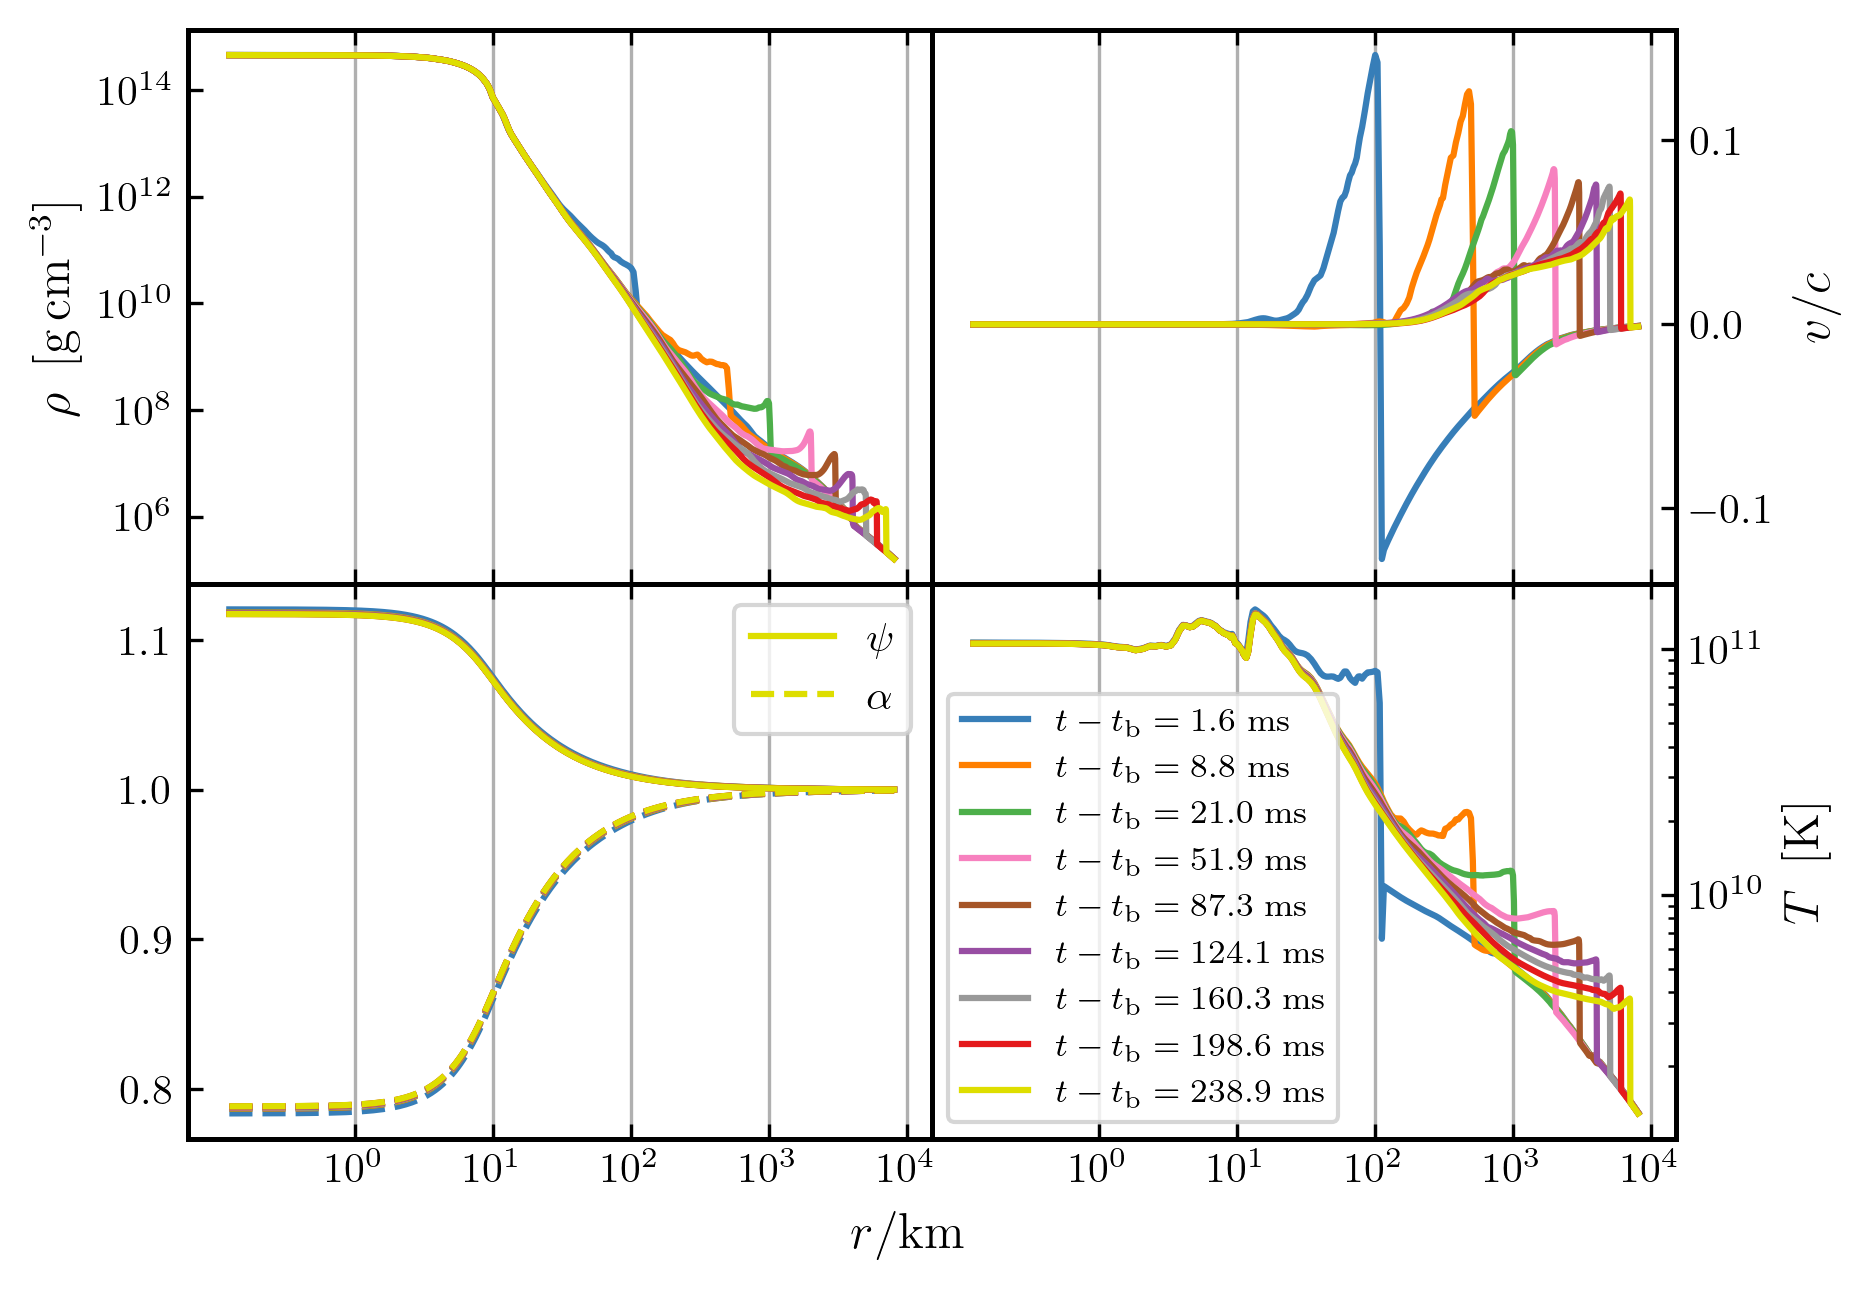
\includegraphics[width=0.8\textwidth]{fig.postBounce.png}
  \end{figure}

\end{frame}

\begin{frame}
\frametitle{Bibliography}

  \Fontvi
  \bibliography{main.bib}

\end{frame}

\begin{frame}
\frametitle{Summary}

  \begin{tabular}{cl}
    \begin{tabular}{l}
      \parbox{0.7\linewidth}%
      {Can run pure hydro problems in GR with AMR}
    \end{tabular}
    \begin{tabular}{c}
      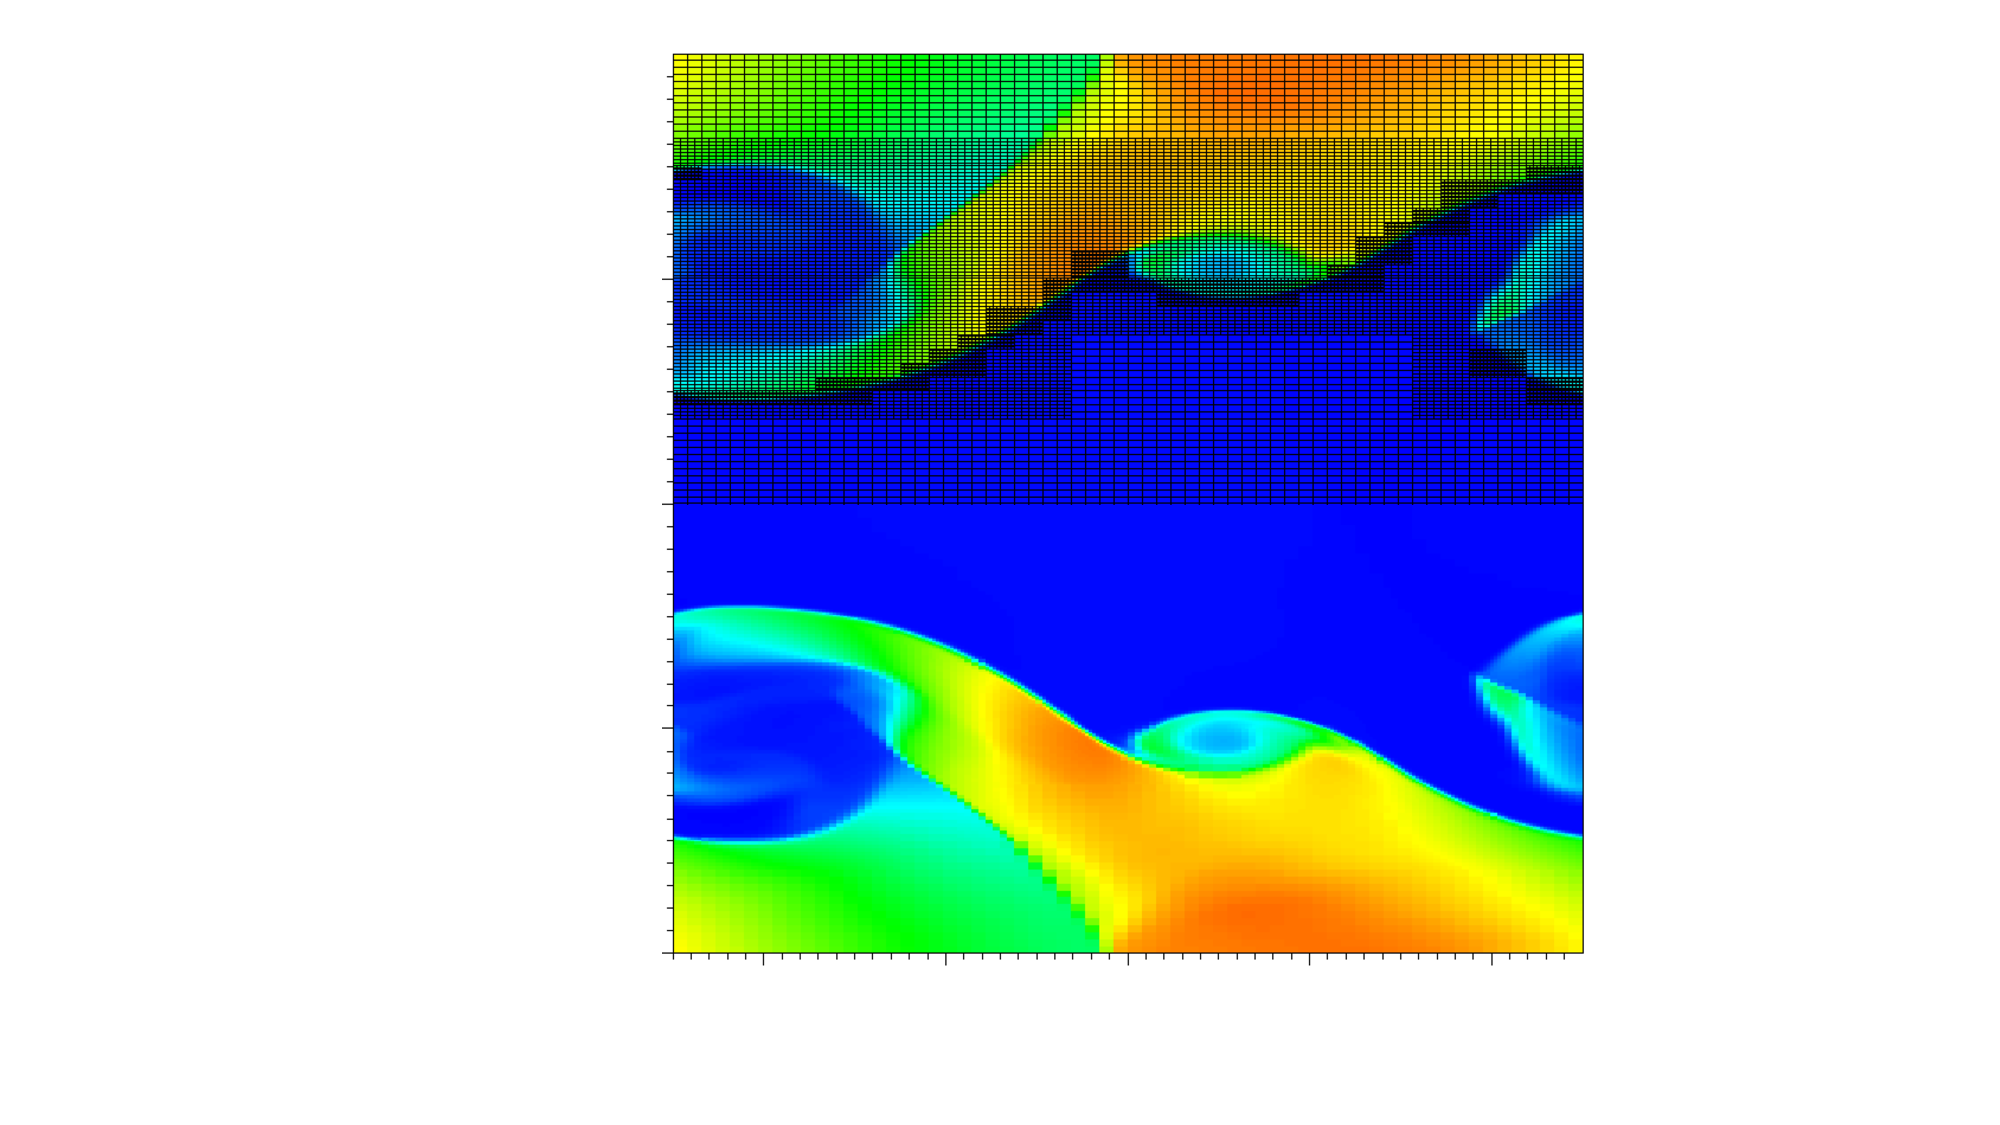
\includegraphics[width=0.15\textwidth]{fig.KHI.pdf}
    \end{tabular}
  \end{tabular}

  \begin{tabular}{cl}
    \begin{tabular}{c}
      \includegraphics[width=0.2\textwidth]{fig.Collapse.png}
    \end{tabular}
    \begin{tabular}{l}
      \parbox{0.7\linewidth}%
      {Can run hydro+self-gravity problems in GR with AMR}
    \end{tabular}
  \end{tabular}

  \begin{tabular}{cl}
    \begin{tabular}{l}
      \parbox{0.7\linewidth}%
      {Working on coupling GR transport to existing hydro+gravity modules}
    \end{tabular}
    \begin{tabular}{c}
      \includegraphics[width=0.2\textwidth]{fig.PostBounce.png}
    \end{tabular}
  \end{tabular}

\end{frame}

\appendix

\begin{frame}
\frametitle{Slope Limiter}

  \Fontvi
  \begin{equation*}
  u_{h}\left(x,t\right)
  =\sum\limits_{n=1}^{N}
  C_{n}\left(t\right)\,P_{n}\left(x\right)\implies
  \tilde{u}_{h}\left(x,t\right)
  =C_{1}\left(t\right)\,P_{1}\left(x\right)
  +\tilde{C}_{2}\left(t\right)\,P_{2}\left(x\right)
  \end{equation*}

  \begin{figure}[htb!]
    \centering
    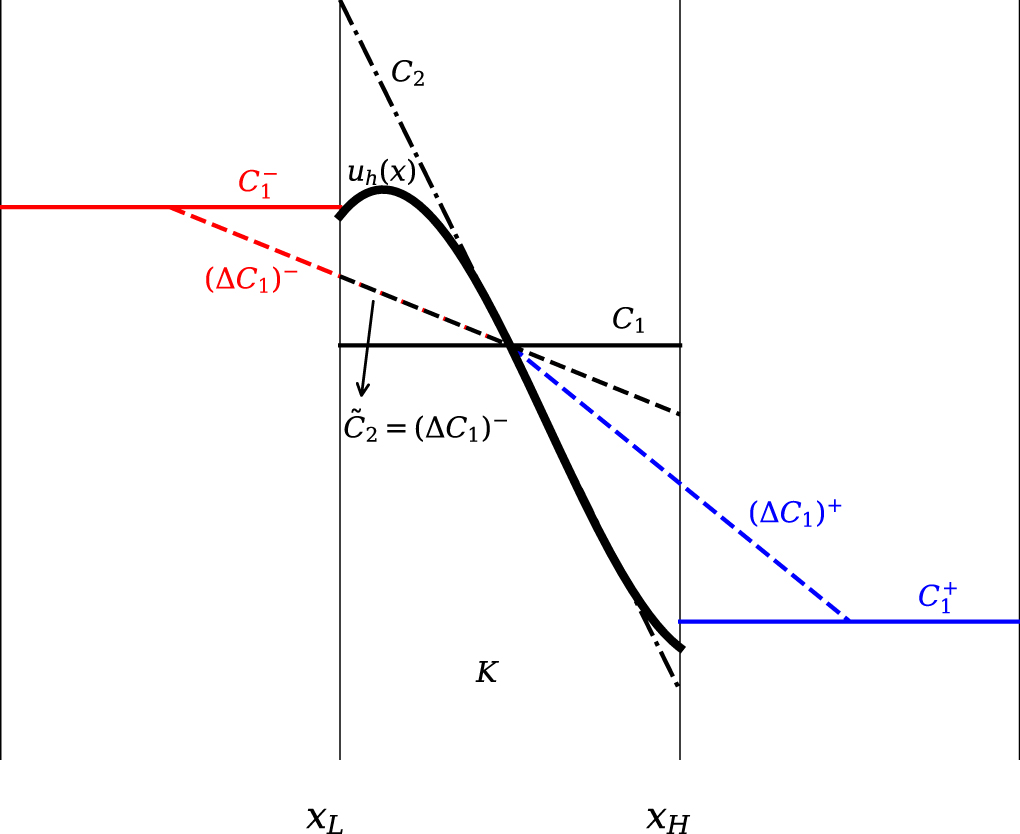
\includegraphics[width=0.6\textwidth]{fig.MinMod.jpeg}
  \end{figure}

\end{frame}

\begin{frame}
\frametitle{3+1 Decomposition}

  \begin{figure}[htb!]
    \centering
    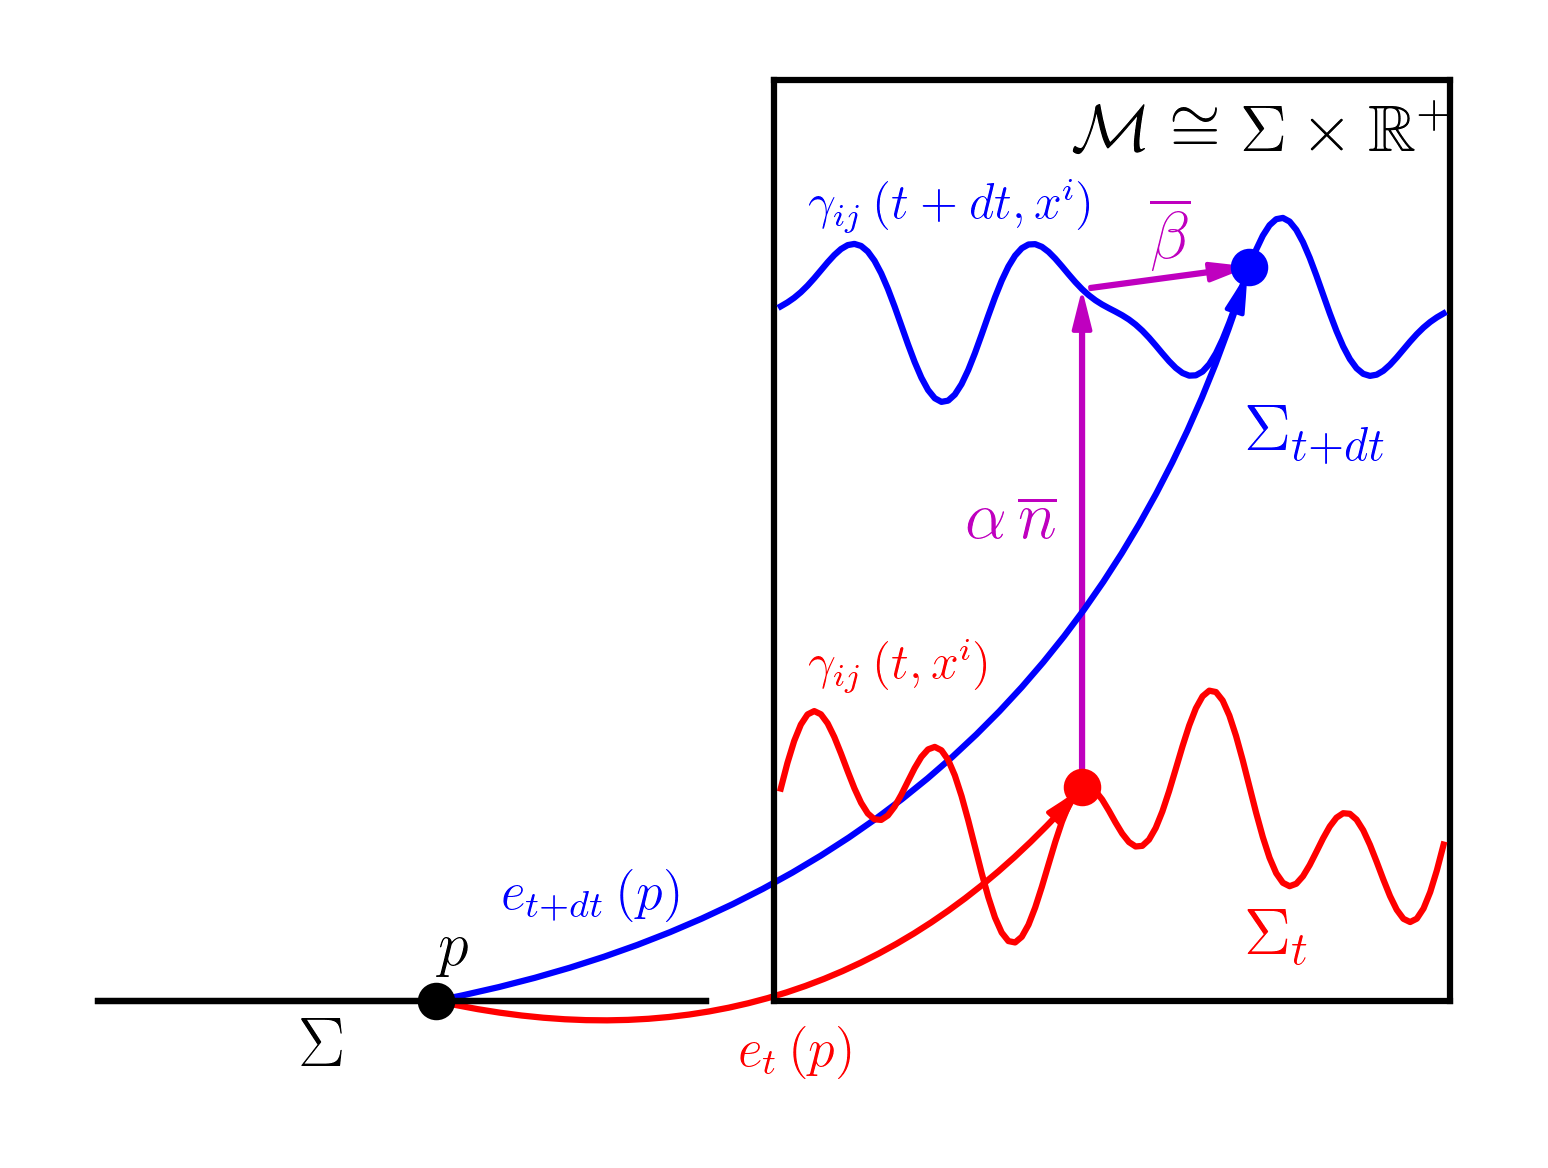
\includegraphics[width=0.7\textwidth]{fig.1p1.png}
  \end{figure}

  \vspace{-2em}

  \begin{equation*}
    ds^{2}
    =g_{\mu\nu}\,dx^{\mu}\,dx^{\nu}
    =-\alpha^{2}\,dt^{2}
     +\gamma_{ij}\left(dx^{i}+\beta^{i}\,dt\right)
                 \left(dx^{j}+\beta^{j}\,dt\right)
  \end{equation*}

\end{frame}

\begin{frame}
\frametitle{Conformally-Flat Condition}

  \begin{columns}[c]

    \column{.5\textwidth}

      Developed by \citet{wmm1996}, extended by \citet{ccd2009}

      \begin{align*}
        \gamma_{ij}\left(x\right)
        &=\psi^{4}\left(x\right)\,\overline{\gamma}_{ij}\left(x^{i}\right) \\
        K&=0,\ \p_{t}\,K=0 \\
        &\hspace{-3em}\mathrm{(Always\ and\ everywhere)}
      \end{align*}\vspace{1em}

      \begin{itemize}
        \item Exact in spherical symmetry!
        \item Hyperbolic $\rightarrow$ Elliptic equations
        \item Good for long-time simulations
      \end{itemize}

    \column{.5\textwidth}

      Special case: Schwarzchild spacetime in isotropic coordinates
      ($G=c=1$)

      \begin{align*}
        \alpha
          &=\left(1+\frac{1}{2}\,\Phi\right)
            \left(1-\frac{1}{2}\,\Phi\right)^{-1} \\
        \psi
          &=1-\frac{1}{2}\,\Phi \\
        \beta^{i}
          &=0,
      \end{align*}
      with
      \begin{equation*}
        \Phi\left(r\right):=-\frac{M}{r}
      \end{equation*}

  \end{columns}

\end{frame}

\end{document}
%------------------------------------------------------------------------------%
